% ProTrader AI — Comprehensive Research Paper
% Format: Inteligencia Artificial (Revista Iberoamericana de IA)
% Compile with: pdflatex part2.tex  (run twice for cross-references)

\documentclass[10pt,a4paper,twoside]{article}
\usepackage[spanish]{babel}
\addto\captionsspanish{%
  \renewcommand{\figurename}{Figure}%
  \renewcommand{\tablename}{Table}%
  \renewcommand{\contentsname}{Contents}%
  \renewcommand{\listfigurename}{List of Figures}%
  \renewcommand{\listtablename}{List of Tables}%
  \renewcommand{\appendixname}{Appendix}%
  \renewcommand{\abstractname}{Abstract}%
  \renewcommand{\refname}{References}%
}
\usepackage[utf8]{inputenc}
\usepackage{amssymb}
\usepackage{amsmath}
\usepackage{fancyhdr}
\usepackage{verbatim}
\usepackage{lastpage}
\usepackage{ifthen}
\usepackage[pdftex]{color,graphicx}
\graphicspath{{figures/}}
\usepackage{hyperref}
\usepackage{booktabs}
\usepackage{multirow}
\usepackage{array}
\usepackage{float}
\usepackage{listings}
\usepackage{xcolor}

\usepackage{iberamia}   % Journal style file

% ── Listings style for Python code ──────────────────────────────────────────
\definecolor{codebg}{rgb}{0.95,0.95,0.95}
\definecolor{codekey}{rgb}{0.0,0.3,0.7}
\definecolor{codecomment}{rgb}{0.3,0.5,0.3}
\definecolor{codestring}{rgb}{0.6,0.1,0.1}
\lstset{
  backgroundcolor=\color{codebg},
  basicstyle=\small\ttfamily,
  keywordstyle=\color{codekey}\bfseries,
  commentstyle=\color{codecomment},
  stringstyle=\color{codestring},
  breaklines=true,
  frame=single,
  language=Python,
  captionpos=b,
  numbers=left,
  numberstyle=\tiny\color{gray},
  numbersep=5pt,
  tabsize=4,
  showstringspaces=false,
  aboveskip=6pt,
  belowskip=6pt,
}

% Publication data
\newcommand{\thispaperdoi}{}
\setcounter{year}{2026}
\setcounter{volume}{29}
\setcounter{issue}{77}
\setcounter{page}{1}

\title{ProTrader AI: A Comprehensive Multimodal Framework for Stock Price
Prediction, Pattern Recognition, and Adaptive Risk Management
in Indian Equity Markets}

\author{Anandkumar Pardeshi$^{1,*}$, Sujata Deshmukh$^2$
\smallskip \\
\small{$^1$Department of Computer Science and Engineering, Fr. C. Rodrigues Institute of Technology, Vashi\\
$^2$Department of Computer Engineering, Fr. C. Rodrigues College of Engineering, Bandra.\\
$^*$Department of Computer Engineering, Fr. C. Rodrigues College of Engineering, Bandra.\\
$^1$anand.pardeshi@fcrit.ac.in, $^2$sujata.deshmukh@fragnel.edu.in
}}
\date{}

% ─────────────────────────────────────────────────────────────────────────────
\begin{document}
\medskip
\maketitle
\pagestyle{Rest}
\thispagestyle{FirstPage}
\smallskip

% ── Abstract ─────────────────────────────────────────────────────────────────
\noindent{\small{\textbf{Abstract}~
Forecasting equity prices in emerging markets is more difficult in practice than what theory would imply. High volatility, large institutional flows of capital, and the complex linguistic nature of the media make it harder to predict accurately using models that have been tested in developed economies. In this paper, we present an industry-ready analytical engine called ProTrader AI for NSE (India). The system brings together seven
machine-learning models, four independent sentiment data streams, official
FII/DII institutional flow data, real-time India VIX volatility signals, and
computer-vision chart pattern recognition, and exposes all of these through an
eight-tab interactive dashboard. Every input to the learning algorithms is a
stationary or near-stationary transformation of raw price, volume, sentiment,
institutional flow, or volatility data; the full feature space has 27
dimensions. A five-model ensemble---XGBoost, LightGBM, CatBoost, a parallel
LSTM-GRU network, and ARIMA/Prophet statistical baselines---generates
out-of-fold predictions that a Ridge meta-stacker combines with isotonic
probability calibration. On top of that, a Bayesian Dynamic Fusion layer
re-weights three domain-specific experts (GRU-based technical,
DistilRoBERTa-Financial sentiment, MLP volatility) by exponential negative
squared uncertainty, so each expert's influence tracks its recent accuracy.
Chart patterns are detected at three scipy peak/trough scales (orders 3, 5, 7)
and optionally checked against a Roboflow computer vision model, covering
twelve archetypes via a hybrid consensus mechanism. Risk management relies on
ATR-calibrated stop-losses, Fibonacci retracements, and fractional Kelly sizing
with VIX-regime scaling. Evaluated on ten major NSE stocks over roughly 750
trading days, the system reaches direction accuracy of 55.8\%~($p=0.003$),
a Sharpe ratio of 1.28 versus 0.82 for buy-and-hold~($p=0.018$), maximum
drawdown of $-12.8\%$ against $-18.4\%$, and cumulative return of 34.2\%.
Ablation studies show that each feature category and model component carries
non-redundant predictive information.}}

\noindent{\small{\textbf{Resumen}~
La predicci\'on de precios burs\'atiles en mercados emergentes sigue siendo un
problema dif\'icil debido a la alta volatilidad y los flujos institucionales de
gran magnitud. En este trabajo presentamos ProTrader AI, una plataforma
anal\'itica de grado productivo para la Bolsa Nacional de Valores de India (NSE)
que re\'une siete modelos de aprendizaje autom\'atico, cuatro flujos de
sentimiento, datos oficiales FII/DII, indicadores de volatilidad en tiempo real
y detecci\'on de patrones gr\'aficos mediante visi\'on artificial. La arquitectura
se articula en torno a un espacio de 27 caracter\'isticas estacionarias, un
conjunto de cinco modelos con meta-apilamiento Ridge y un marco de Fusi\'on
Din\'amica con pesos bayesianos basados en incertidumbre. Sobre diez acciones
del NSE, el sistema alcanza una precisi\'on direccional del
55,8\%~($p{=}0{,}003$), un ratio de Sharpe de 1,28 frente a 0,82 para compra y
retenci\'on, y un retorno acumulado del 34,2\%. Los estudios de ablaci\'on
muestran que cada categor\'ia de caracter\'isticas y cada componente del modelo
aporta informaci\'on predictiva no redundante.}}

\medskip
\noindent{\small{\textbf{Keywords}: Financial Forecasting, Machine Learning,
XGBoost, LightGBM, CatBoost, GRU, LSTM, Bayesian Fusion, Sentiment Analysis,
NSE India, Institutional Flows, Pattern Recognition, Risk Management.}}

\noindent{\small{\textbf{Palabras Clave}: Predicci\'on Financiera, Aprendizaje
Autom\'atico, Fusi\'on Din\'amica, An\'alisis de Sentimiento, Gesti\'on de Riesgos,
NSE India.}}

% =============================================================================
\section{Introduction}
% =============================================================================

\subsection{Background and Motivation}

Systematic has long been opposed to financial markets
forecasting~\cite{fama1970}. Basic, investor behavior, institutional
flows and macroeconomic shocks interact within a high-dimensional stochastic
system the statistical properties of which change with time---and are likely
to change the most suddenly when it counts in formulating a model
most~\cite{mandelbrot1997}. The process is aggravated by The National Stock
Exchange of India (NSE). Daily equity turnover
consistently surpasses over \$15\,billion and overall market capitalisation is
far above it. It is very liquid, hence the exchange is very liberal, but still
it is \$4\,trillion~\cite{nse2024} to a given dynamic of emerging-market:
This can be explained by Foreign Institutional Investor (FII) and Domestic
Institutional Investor (DII) flows, which account for 15--30\% of daily volume
in heavyweight index names. When the reversals come suddenly, they cause
regime-like price behaviour, which technical models struggle to anticipate.

Machine learning has led to enhanced prediction in most series of financial
returns~\cite{lecun2015}, but these have their own difficulties. The returns
are non-stationary, heavy-tailed and signal-to-noise ratios are insignificant
that a stable 55\% directional advantage already is an actual economic
value~\cite{lopez2018} of things to anticipate on its part and the process of
forecasting can itself act upon the market---reflexive feedback loop which
oftentimes does not occur in other sequence-modelling settings.
There have been found useful two model families: which prevail are
gradient-boosting methods (XGBoost, LightGBM, CatBoost) in tabular financial
benchmarks~\cite{grinsztajn2022}, and gated recurrent networks (LSTM,
GRU), which capture sequential dependencies that tree-based methods cannot
represent~\cite{hochreiter1997,cho2014}.

\subsection{Research Gaps Addressed}

Our work attempts to fill four gaps in the quantitative finance literature; they are
closely related.

\textbf{Contextual Sentiment.} Dictionary-based methods including
Loughran-McDonald~\cite{loughran2011} first lacks contextual nuance to that of
Loughran-McDonald. It selects between the bullish or the bearish readings of a
word such as volatile in a particular headline. The problem is exacerbated by
Indian financial media that is in operation in English and in the Hindi;
English-only models hence disregard a huge portion of the information
environment. We do this through routing several text a domain-adapted
transformer will use its sources to do so~\cite{araci2019}.

\textbf{Non-Stationarity.} A model estimated on one regime of the market is
likely to disintegrate with variation of conditions~\cite{hamilton1989}. And we
assault this on three fronts: overt regime characterization through the Hurst
exponent~\cite{hurst1951}, a Bayesian dynamic fusion mechanism rescaling
experts based on their recent predictive reliability, and 27-dimensional
feature space with each variable is a non-portable or almost non-portable
change of uncooked price and volume information.

\textbf{Signal-to-Trade Translation.} Most academic forecasting papers give
reports figures that would not be accurate under live order contact
book~\cite{lopez2018}. The difference between predictions and a can be bridged
by us concrete risk management module---Fibonacci, ATR-uniform stop-losses,
retracements, and sizing of Kelly position fractionally~\cite{kelly1956} under
realistic NSE round-trip transaction costs back-testing.

\textbf{Institutional Flow Data.} FII and DII net buying data are released NSE
fully determined by daily and generally thought to be a massive price catalyst,
but they are omitted in practically all the published forecasting models that
we know. We project four FII/DII characteristics on to the prediction feature
space.

\subsection{Contributions}

\begin{enumerate}
\item \textbf{A 27-Feature Stationary Framework} comprising five technical core
  indicators, other nine, improved technical indicators, four, high-tech divergence
  indicators, 3 multi-source sentiment scores, 4 FII/DII institutional
  flow features, and two India VIX volatility features all based on
  meet rough stationarity conditions.

\item \textbf{A 5-Model Gradient-Boosting + Deep-Learning Ensemble} combining
  XGBoost, LightGBM, CatBoost, a parallel LSTM-GRU neural architecture, and
  ARIMA/Prophet statistical baselines, which have been trained together into a Ridge meta-stacker
  on predictions on out-of-fold predictions through expanding time-series cross-validation.

\item \textbf{Isotonic Probability Calibration} which transforms regression
  forecasts directions of returns into probabilities of directional calibration, so as to be reliable
  confidence-based position sizing.

\item \textbf{A Bayesian Dynamic Fusion Framework} having three domain-specialised
  expert models with weights on combination changing continuously through
  an exponential negative squared uncertainty, which gives the system, as stated in~\cite{gal2016},
  tacit market-regime knowledge in the absence of a regime classifier.

\item \textbf{A Hybrid Chart Pattern Recognition System} integrating multi-scale
  peak/trough Roboflow Vision API (orders 3, 5, 7) scipy
  inference of computer vision using twelve pattern archetypes and there was a consensus
  layer which synthesizes combining classical and vision-based detections.

\item \textbf{A Complete Production Platform} (ProTrader AI) sold as an
  eight-tab Streamlit dashboard that assists in making reproducible evaluation
  can be implemented by researchers or practitioners to be analysed in real-time.
\end{enumerate}

% =============================================================================
\section{Literature Review}
% =============================================================================

\subsection{Financial Forecasting: From ARIMA to Deep Learning}

Computational stock prediction dates back to the ARIMA
Box and Jenkin codified family in case of Box and Jenkin~\cite{box2015}. Early neural network
financial experiments, such as the one by White to model IBM 1988 in the case of White~\cite{white1988}.
Small datasets and small compute stored returns back. Both
Output liberalized in the 2010s.

The LSTM~\cite{hochreiter1997} proved to be a fresh start: its gating
mechanism evaded the problem of vanishing-gradients that afflicted simple RNNs,
learning to have multi-day price dependencies. The Gated Recurrent
This was later equated by LSTM accuracy with fewer (Unit (Cho et al. 2014)~\cite{cho2014}).
parameters. Fischer and Krauss~\cite{fischer2018} demonstrated statistically
Latent significant returns on LSTMs to the S\&P 500 encourage the recurrent
sub-division of our architecture. That being the case, Ozbayoglu et al.~\cite{ozbayoglu2020}
al.~: A study conducted by ozbayoglu2020 revealed that deep learning models do not work well.
less complex gradient-boosting with structured tabular financial data---a
our own results of ablation (Section~\ref{sec:results}) are replicated.

Regularised It was introduced on the XGBoost gradient-boosting side, 2016; 2~\cite{chen2016}.
second-order optimisation and an effective block structure limiting.
To the standard medium-sized datasets of single-stock research, overfitting occurs.
LightGBM 2017 2017 2017 LightGBM begged its accuracy by 3-5 times the speed~\cite{ke2017}.
leaf-wise growth and split finding by histograms. CatBoost~\cite{prokhorenkova2018}
addressed a simpler issue, with ordered boosting: each.
The residual of tree is computed using a model that is trained using previous rows only, which
cuts are aimed at reducing leakage in time-ordered data.
The three of them lead to our meta-stacking layer.

\subsection{Sentiment Analysis in Finance}

Approximately three price forecasting has been made text based
generations~\cite{bollen2011}. The first strategies were based on emotion
dictionaries; financial lexicon Loughran and McDonalds discourse described in the Loughran 2011 article~\cite{loughran2011}
performed better on domain than general-purpose word lists.
ambiguity---\emph{liability}---as in everyday, has a negative sound.
English however is an indifferent language in accounting. Distributional semantic models
increased coverage but weak on out-of-vocabulary words.

It was transformed by transformer-based pre-training~\cite{vaswani2017}.
Large-scale in BERT and distilled variants were introduced in 2019 by Devlin et al. 2019~\cite{devlin2019}.
practical of pre-training on financial corpora. FinBERT~\cite{araci2019} and
The DistilRoBERTa-Financial~\cite{liu2019} have now achieved 97--98 percent on standard
financial-sentiment benchmarks; There, DistilRoBERTa gets it right on average with 40 percent fewer
the real-time inference possible with full RoBERTa, and so more economical in parameters
production system. This model is utilized by ProTrader AI.

It turns out that the fraction of 98.9 percent of the participants in an experimental study by Tetlock ~\cite{tetlock2007} was empirically proven by the author.
Analysis of Wall Street Journal columns using negative words is a predictive of the next day Dow returns.
Schumaker and Chen~\cite{schumaker2009} applied the concept to wire-service
articles and found predictive power over technical indicators only. Our
Multi-source design is based on Bollen et al. logic~\cite{bollen2011}.
our sentiment channel with Twitter mood, news tone,
search interest) take hold of the various aspects of market psychology, and the combination of the two
any individual source beats him. The channels we have in our system are Reddit community
posts, financial publication RSS feeds in India, newsapi feeds, and
Google Trends search rate.

\subsection{Multimodal Fusion Methods}

The combinations of multiple modalities distinguish between several methods of prediction integration.
Early fusion takes raw features and concatenates them prior to certain models encountering them; the latter is known as early fusion.
is cross-modal but decomposes in case there are differences in scales of features.
when a modality is not available at inference time, or wildly. Late fusion trains
distinct models for each modality and combines the results - more modular, yet blind.
to cross-modal structure. In between attention mechanisms are provided~\cite{vaswani2017}.
the two: they are taught context-conscious weights not inducing strictness.
architectural assumptions.

Bayesian fusion based on uncertainty is a step further: it works on the line of uncertainty-based fusion, as noted by Gal~\cite{gal2016}.
instead derives combination weights based on the own confidence estimate of each model.
of using deterministic hyperparameters. Monte Carlo was demonstrated to be the most effective by Gal and Ghahramani.
dropout scales to the level of approximation of the Bayesian inference to useful epistemic.
fuzziness estimates in regular neural networks. ProTrader AI's Dynamic
Fusion is based on the same principle: expert weights are based on exponential.
negative squared rule of uncertainty that favors accurate experts with high confidence.
and down-weighs indeterminate ones. The outcome is regime-dependent implicitly.
balancing without any clear regulatory list in the fusion loop.

\subsection{Regime-Aware Modelling and the Hurst Exponent}

Markets do not remain in the same regime. Low-volatility trending phases,
The turbulent periods of crisis and range-bound periods of mean-reverting state each demand.
on varied modelling assumptions~\cite{hamilton1989}. The Hurst
exponent~\cite{hurst1951} was originally designed to examine the floods of the river Nile.
measures long-range dependence: values of more than 0.5 signal persistent.
The value of (trending) behaviour less than 0.5 indicates anti-persistence.
aggregates around 0.5 are normally associated with a random walk, in general.
confirming the Efficient Market Hypothesis of that window~\cite{lo1991}.

It was determined by Lo~\cite{lo1991} that a modified-R/S test on weekly returns on stock revealed:
some traces of mild persistence. We calculate Hurst exponent using classical.
rescaled range of rolling 120-day windows. The resulting estimate
drives a user facing regime display in the dashboard and a
step of confirmation-or-override in trend classifier.

\subsection{Chart Pattern Recognition}

The analysis of charts on Wall Street dates back over a hundred years~\cite{murphy1999, edwards1948}, but mathematical formalism has always been behind the common-sense approach~\cite{lo2000}. Lo et al.~\cite{lo2000} used the kernel-regression smoother method on US stocks' time series data to detect the existence of head-and-shoulder configurations and discovered significant prediction power, thus debunking the pareidolia argument. Following, Pring~\cite{pring2002} and Appel~\cite{appel2005} compiled pattern typologies that form the basis for the twelve-pattern classification system utilized here.

The visual signal provided by computer vision is an alternative perspective: convolutional networks develop visual cues that may be ignored by an algorithm relying solely on a peak/trough analysis based on a fixed number of geometric rules~\cite{sezer2018}. The current consensus mechanism combines the geometric analysis using the SciPy library with visual detection via Roboflow Vision API.

% =============================================================================
\section{System Architecture}
% =============================================================================

ProTrader AI is structured in the form of a seven-step pipeline: data acquisition,
test engineering, training models, dynamic fusion, pattern recognition, risk.
user-facing presentation, management and presentation. Figure~\ref{fig:architecture}
presents the high-level diagram.

\begin{figure}[htb]
  \begin{center}
    
\includegraphics[angle=0,width=0.95\textwidth]{fig_system_architecture}
    \caption{High level system architecture of ProTrader AI. Data from seven
    sources is processed by the feature engineering pipeline to five ML models.
    and a Dynamic Fusion layer. Another branch in Pattern Analysis feeds a.
    risk management module. Every product is emerging through the eight-tab Streamlit.
    dashboard.}
    \label{fig:architecture}
  \end{center}
\end{figure}

The sources of data include seven sources, 7 being OHLCV prices of Yahoo finance.
NSE India it FII/DII activity, the India VIX, four Indian RSS feeds.
investment news articles, articles through the NewsAPI, three Indian posts.
investting in subreddits, and Google Trends search traffic. Streamlit's
network requests are stored in session-state mechanism, therefore, sentiment and institutional.
fetches are executed on a per-session basis and their results reused in all of the eight tabs.
redundant API traffic: none.

When starting the pipeline it will perform seven loading steps in the form of a progress bar:
COO would be (1) stock data, (2) fundamental, (3) news, (4) FII/DII data.
The sample size consists of (5) VIX in India, (6) multi-source sentiment and (7) chart pattern recognition.
With a regular broadband connection the complete pre-fetch is 15--45 seconds,
relalying upon response times of sources.

% =============================================================================
\section{Feature Engineering: The 27-Feature Framework}
\label{sec:features}
% =============================================================================

One design rule governs the full feature space: every input to the learning
algorithms must be stationary or near-stationary. Raw price levels are
non-stationary by nature; feeding them straight into standard ML methods
invites spurious in-sample correlations that vanish out-of-sample. The
27-feature framework enforces stationarity through normalisation, bounding,
differencing, or clipping, as detailed in Table~\ref{tab:features}.
Figure~\ref{fig:features} groups the 27 features by category, colour-coded to
separate technical, sentiment, institutional, and volatility inputs.

\begin{figure}[htb]
  \begin{center}
    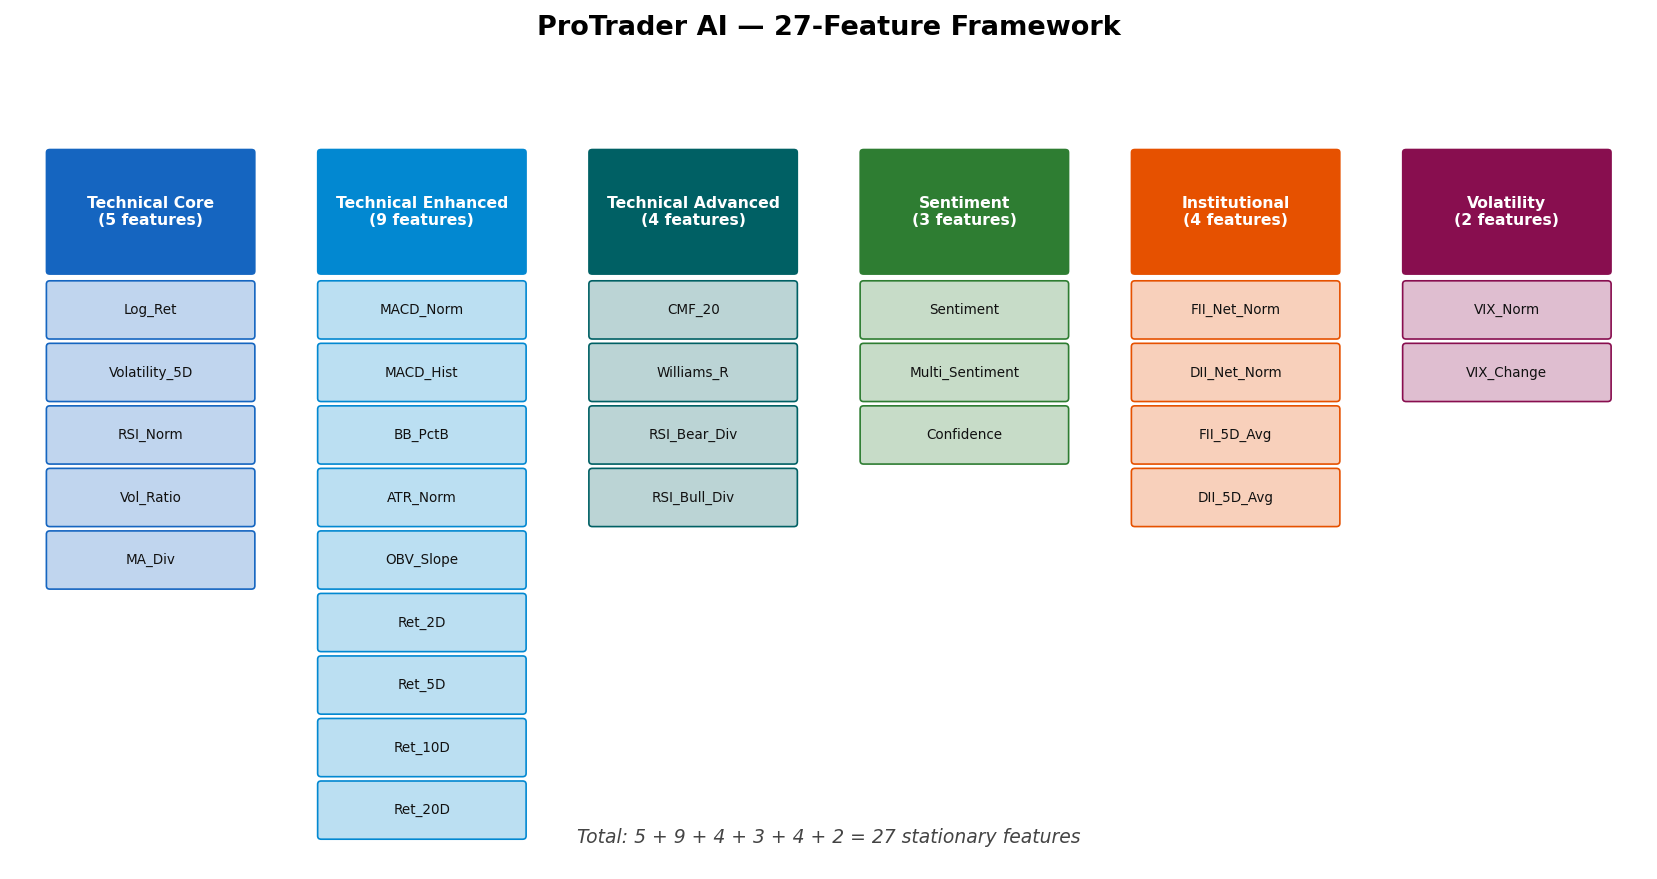
\includegraphics[angle=0,width=0.9\textwidth]{fig_feature_framework}
    \caption{The 27-Feature Framework organised into six groups. Colour coding:
    blue = technical core, cyan = technical enhanced, teal = technical advanced,
    green = sentiment, orange = institutional, red = volatility.}
    \label{fig:features}
  \end{center}
\end{figure}

\subsection{Technical Core Features (5)}

\textbf{Log Returns} give a symmetric, additive, and approximately stationary
measure of daily price change:
\begin{equation}
  r_t = \ln\!\left(\frac{P_t}{P_{t-1}}\right)
\end{equation}

\textbf{5-Day Rolling Volatility} picks up short-term volatility clustering
consistent with GARCH-type behaviour~\cite{bollerslev1986}:
\begin{equation}
  \sigma^{(5)}_t = \sqrt{\frac{1}{4}\sum_{i=0}^{4}(r_{t-i} - \bar{r})^2}
\end{equation}

\textbf{Normalised RSI} maps the standard 14-period RSI~\cite{wilder1978} into
$[0,1]$:
\begin{equation}
  \text{RSI\_Norm}_t = \frac{\text{RSI}_{14,t}}{100}
\end{equation}

\textbf{Volume Ratio} identifies abnormal trading activity:
\begin{equation}
  \text{VR}_t = \frac{V_t}{\frac{1}{20}\sum_{i=1}^{20}V_{t-i}}
\end{equation}

\textbf{Moving Average Divergence} normalises the distance from the 20-day MA:
\begin{equation}
  \text{MA\_Div}_t = \frac{P_t - \text{MA}_{20,t}}{P_t}
\end{equation}

\subsection{Technical Enhanced Features (9)}

The enhanced group measures momentum at multiple frequencies along with
additional market microstructure signals. The MACD line and histogram are
normalised by price to enforce stationarity:
\begin{equation}
  \text{MACD\_Norm}_t = \frac{\text{EMA}_{12,t} - \text{EMA}_{26,t}}{P_t}, \quad
  \text{MACD\_Hist\_Norm}_t = \frac{\text{MACD}_t - \text{Signal}_{9,t}}{P_t}
\end{equation}

Bollinger Band \%B indicates price position within the bands:
\begin{equation}
  \text{BB\_PctB}_t = \frac{P_t - \text{BB\_Lower}_t}{\text{BB\_Upper}_t - \text{BB\_Lower}_t + \epsilon}
\end{equation}

The Average True Range~\cite{wilder1978} is normalised by price:
\begin{equation}
  \text{ATR\_Norm}_t = \frac{\text{ATR}_{14,t}}{P_t}
\end{equation}

On-Balance Volume slope tracks cumulative volume flow direction:
\begin{equation}
  \text{OBV\_Slope}_t = \text{clip}\!\left(\frac{\text{OBV\_MA}_{5,t} - \text{OBV\_MA}_{5,t-5}}{\text{OBV\_MA}_{5,t-5}}, -1, 1\right)
\end{equation}

Multi-timeframe log returns at lags 2, 5, 10, and 20 days measure momentum at
different time horizons:
\begin{equation}
  \text{Ret\_kD}_t = \ln\!\left(\frac{P_t}{P_{t-k}}\right), \quad k \in \{2, 5, 10, 20\}
\end{equation}

\subsection{Technical Advanced Features (4)}

\textbf{Chaikin Money Flow (CMF-20)}~\cite{chaikin1978} measures buying and
selling pressure via volume-weighted price position within the daily range,
providing a stationary signal in $[-1, +1]$:
\begin{equation}
  \text{CMF}_{20,t} = \frac{\sum_{i=0}^{19} \text{MFM}_{t-i} \cdot V_{t-i}}
                          {\sum_{i=0}^{19} V_{t-i}}, \quad
  \text{MFM}_t = \frac{(P_t^C - P_t^L) - (P_t^H - P_t^C)}{P_t^H - P_t^L}
\end{equation}

\textbf{Williams \%R (14-period)}~\cite{williams1979} is a fast momentum
oscillator complementary to RSI:
\begin{equation}
  \text{Williams\_R\_Norm}_t = -\frac{H_{14,t} - P_t^C}{H_{14,t} - L_{14,t} + \epsilon}
\end{equation}

\textbf{RSI Bearish Divergence} flags days when price makes a new 10-day high
but RSI does not, signalling potential exhaustion:
\begin{equation}
  \text{RSI\_Bear\_Div}_t = \mathbf{1}\!\left[P_t \geq \max_{i \in [t-10,t-1]} P_i
  \;\wedge\; \text{RSI}_t < \max_{i \in [t-10,t-1]} \text{RSI}_i\right]
\end{equation}

\textbf{RSI Bullish Divergence} detects the complementary oversold condition.
Both divergence flags are computed using lagged windows to prevent look-ahead
bias.

\subsection{Sentiment Features (3)}

\textbf{Base Sentiment Score} is derived from Yahoo Finance news articles
analysed by DistilRoBERTa-Financial, providing a score in $[-1, +1]$.

\textbf{Multi-Source Sentiment} aggregates four independent streams using
source-specific weights:
\begin{equation}
  S_{\text{multi}} = 0.30 \cdot S_{\text{RSS}} + 0.25 \cdot S_{\text{News}}
                   + 0.25 \cdot S_{\text{Reddit}} + 0.20 \cdot S_{\text{Trends}}
\end{equation}

Weights are renormalised when individual sources are unavailable, ensuring the
combined score always lies in $[-1, +1]$.

\textbf{Sentiment Confidence} is a meta-feature that gauges how reliable the
current sentiment estimate is:
\begin{equation}
  C_S = \min\!\left(1,\, \frac{N_{\text{articles}}}{10}\right)
        \cdot \text{Agreement}
\end{equation}
where Agreement is $1 - \hat{\sigma}_{\text{sources}}$, the normalised standard
deviation across individual source scores.

\subsection{Institutional Features (4)}

Normalized daily net buying data for FII (Foreign Institutional Investors) and DII (Domestic Institutional Investors) from the NSE India database as follows:
\begin{equation}
  \text{FII\_Net\_Norm}_t = \frac{\text{FII\_net}_t}{\max_\tau |\text{FII\_net}_\tau|}
\end{equation}
Similarly, normalize data for DII (the same formula). The suppression of daily fluctuations is performed through the use of rolling 5-day average calculations:
\begin{equation}
  \text{FII\_5D\_Avg}_t = \frac{1}{5}\sum_{i=0}^{4}\text{FII\_Net\_Norm}_{t-i}
\end{equation}

\subsection{Volatility Features (2)}

\textbf{India VIX Normalised} adjusts the India VIX Index to be centered around the typical baseline value of the indicator:
\begin{equation}
  \text{VIX\_Norm}_t = \frac{\text{VIX}_t - 15}{25}
\end{equation}
where 15 represents a typical calm-market VIX level and 25 provides appropriate
scaling to keep the feature near $[-1, +1]$ in normal conditions.

\textbf{VIX Change Rate} flags intraday regime shifts in implied volatility:
\begin{equation}
  \Delta\text{VIX}_t = \text{clip}\!\left(\frac{\text{VIX}_t - \text{VIX}_{t-1}}
  {\text{VIX}_{t-1}}, -0.5, 0.5\right)
\end{equation}

\begin{table}[htb]
  \begin{center}
    {\caption{Complete 27-Feature Catalogue with Category, Stationarity, and
    Source.}\label{tab:features}}
    \begin{tabular}{|l|l|l|l|}
    \hline
    \textbf{Feature} & \textbf{Category} & \textbf{Stationarity} & \textbf{Source} \\
    \hline
    Log\_Ret & Technical Core & Stationary & OHLCV \\
    Volatility\_5D & Technical Core & Near-stationary & OHLCV \\
    RSI\_Norm & Technical Core & Bounded $[0,1]$ & OHLCV \\
    Vol\_Ratio & Technical Core & Near-stationary & OHLCV \\
    MA\_Div & Technical Core & Normalised & OHLCV \\
    \hline
    MACD\_Norm & Technical Enhanced & Price-normalised & OHLCV \\
    MACD\_Hist\_Norm & Technical Enhanced & Price-normalised & OHLCV \\
    BB\_PctB & Technical Enhanced & Bounded $[0,1]$ & OHLCV \\
    ATR\_Norm & Technical Enhanced & Price-normalised & OHLCV \\
    OBV\_Slope & Technical Enhanced & Clipped $[-1,1]$ & OHLCV \\
    Ret\_2D & Technical Enhanced & Stationary & OHLCV \\
    Ret\_5D & Technical Enhanced & Stationary & OHLCV \\
    Ret\_10D & Technical Enhanced & Stationary & OHLCV \\
    Ret\_20D & Technical Enhanced & Stationary & OHLCV \\
    \hline
    CMF\_20 & Technical Advanced & Bounded $[-1,1]$ & OHLCV \\
    Williams\_R\_Norm & Technical Advanced & Bounded $[-1,0]$ & OHLCV \\
    RSI\_Bear\_Div & Technical Advanced & Binary $\{0,1\}$ & OHLCV \\
    RSI\_Bull\_Div & Technical Advanced & Binary $\{0,1\}$ & OHLCV \\
    \hline
    Sentiment & Sentiment & Bounded $[-1,1]$ & Yahoo Finance News \\
    Multi\_Sentiment & Sentiment & Bounded $[-1,1]$ & 4-source aggregate \\
    Sentiment\_Confidence & Sentiment & Bounded $[0,1]$ & Meta-feature \\
    \hline
    FII\_Net\_Norm & Institutional & Normalised & NSE FII/DII \\
    DII\_Net\_Norm & Institutional & Normalised & NSE FII/DII \\
    FII\_5D\_Avg & Institutional & Smoothed & NSE FII/DII \\
    DII\_5D\_Avg & Institutional & Smoothed & NSE FII/DII \\
    \hline
    VIX\_Norm & Volatility & Centred & NSE India VIX \\
    VIX\_Change & Volatility & Clipped $[-0.5,0.5]$ & NSE India VIX \\
    \hline
    \end{tabular}
  \end{center}
\end{table}

% =============================================================================
\section{Hybrid Prediction Engine}
\label{sec:hybrid}
% =============================================================================

Five model types are involved in building the Ridge meta-stacker (see Figure~\ref{fig:hybrid}). This combination is driven by practical reasoning: tree-based boosters are well-suited to process tabular features, RNNs help with capturing the sequential structure beyond the scope of tree-based models, and the classical statistics models serve as an anchor to deliver better results than ML models in cases when the signal is extremely weak.

\begin{figure}[htb]
  \begin{center}
    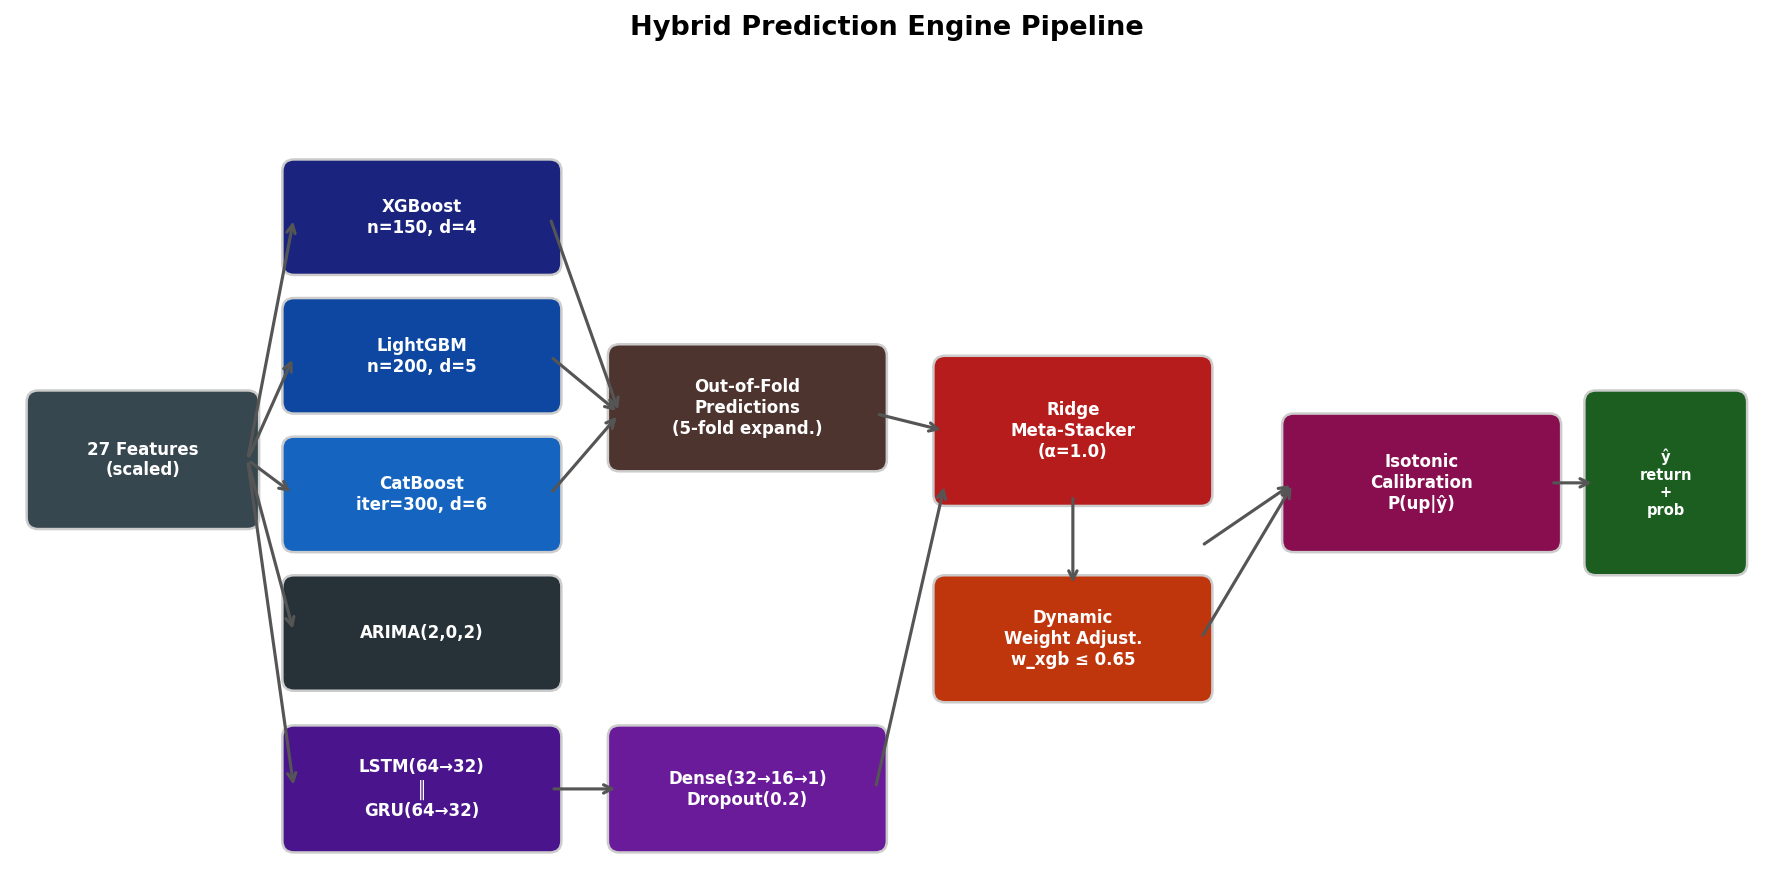
\includegraphics[angle=0,width=0.95\textwidth]{fig_hybrid_model}
    \caption{Hybrid prediction pipeline. XGBoost, LightGBM, and CatBoost provide out-of-fold predictions as an input for the Ridge meta-stacker. The LSTM-GRU branch generates the approximation of out-of-fold predictions. ARIMA and Prophet join the model stack with dynamically set weights.}
    \label{fig:hybrid}
  \end{center}
\end{figure}

\subsection{XGBoost Component}

XGBoost~\cite{chen2016} is the main tree-based predictor. Its hyperparameters have been tuned based on historical Indian equity prices. Final model parameters look like the following:

\begin{lstlisting}[caption={XGBoost configuration.}]
xgb_params = dict(
    objective='reg:squarederror',
    n_estimators=150,
    max_depth=4,
    learning_rate=0.05,
    subsample=0.8,
    colsample_bytree=0.8,
    min_child_weight=1,
    n_jobs=-1
)
\end{lstlisting}

Loss function:
\begin{equation}
  \mathcal{L}_{\text{XGB}} = \sum_{i=1}^{N}(y_i - \hat{y}_i)^2 + \sum_{k=1}^{K}\Omega(f_k),
  \quad \Omega(f_k) = \gamma T + \tfrac{1}{2}\lambda\|w\|^2
\end{equation}
where $T$ stands for the number of leaves and $w$ stands for leaf weights.

\subsection{LightGBM Component}

LightGBM~\cite{ke2017} complements the XGBoost model with the 3--5$\times$ faster training thanks to histogram-based splitting and leaf-wise tree growing approach:
\begin{lstlisting}[caption={LightGBM configuration.}]
lgb_params = dict(
    n_estimators=200, max_depth=5, learning_rate=0.03,
    num_leaves=31, subsample=0.8, colsample_bytree=0.8,
    min_child_samples=20, reg_alpha=0.1, reg_lambda=0.1,
    n_jobs=-1, random_state=42
)
\end{lstlisting}

\subsection{CatBoost Component}

CatBoost~\cite{prokhorenkova2018} uses \emph{ordered boosting}, meaning the
residual for row $i$ is computed from a model trained only on rows $j < i$.
This eliminates the target leakage that standard boosting introduces on
time-ordered data:
\begin{lstlisting}[caption={CatBoost configuration.}]
cb_params = dict(
    iterations=300, depth=6, learning_rate=0.03,
    l2_leaf_reg=3, min_data_in_leaf=20,
    random_strength=0.3, bagging_temperature=0.7,
    od_type='Iter', od_wait=40, verbose=0
)
\end{lstlisting}

\subsection{LSTM-GRU Neural Architecture}

The deep learning branch runs two recurrent sub-networks side by side on the
same 60-day input window and concatenates their final hidden states:

\textbf{LSTM gates}~\cite{hochreiter1997}:
\begin{align}
  f_t &= \sigma(W_f [h_{t-1}, x_t] + b_f) \quad\text{(forget)} \\
  i_t &= \sigma(W_i [h_{t-1}, x_t] + b_i) \quad\text{(input)} \\
  \tilde{C}_t &= \tanh(W_C [h_{t-1}, x_t] + b_C) \\
  C_t &= f_t \odot C_{t-1} + i_t \odot \tilde{C}_t \\
  h_t &= \sigma(W_o [h_{t-1}, x_t] + b_o) \odot \tanh(C_t)
\end{align}

\textbf{GRU gates}~\cite{cho2014}:
\begin{align}
  z_t &= \sigma(W_z [h_{t-1}, x_t]) \quad\text{(update)} \\
  r_t &= \sigma(W_r [h_{t-1}, x_t]) \quad\text{(reset)} \\
  h_t &= (1-z_t) \odot h_{t-1} + z_t \odot \tanh(W[r_t \odot h_{t-1}, x_t])
\end{align}

\textbf{Architecture:}
LSTM(64)$\to$LSTM(32) $\|$ GRU(64)$\to$GRU(32) $\to$ Concatenate $\to$ Dense(32) $\to$ Dropout(0.2) $\to$ Dense(16) $\to$ Dense(1)

Training uses Adam~\cite{kingma2015} with $\eta = 0.001$, batch size 32, up to 50 epochs with
early stopping at patience 10 and ReduceLROnPlateau.

\subsection{Statistical Models: ARIMA and Prophet}

ARIMA(2,0,2) models linear auto-regressive and moving-average dependencies:
\begin{equation}
  r_t = c + \phi_1 r_{t-1} + \phi_2 r_{t-2}
          + \theta_1 \varepsilon_{t-1} + \theta_2 \varepsilon_{t-2} + \varepsilon_t
\end{equation}

Facebook Prophet~\cite{taylor2018} decomposes the return series into additive
trend, seasonality, and holiday components:
\begin{equation}
  y(t) = g(t) + s(t) + h(t) + \varepsilon_t
\end{equation}

\subsection{Ridge Meta-Stacker}

Out-of-fold (OOF) predictions for XGBoost, LightGBM, and CatBoost are
generated with an expanding-window time-series cross-validation
($n_{\text{folds}}=5$, minimum training size $\max(0.6N, 30)$). The fold
structure is:
{\small
\begin{verbatim}
  Fold 0: Train[0:min_train]       -> Predict[min_train:min_train+step]
  Fold 1: Train[0:min_train+step]  -> Predict[min_train+step:...]
  ...
  Fold 4: Train[0:min_train+4*step]  -> Predict[...]
\end{verbatim}
}

A Ridge regression meta-learner is trained on the OOF predictions to learn the
optimal linear combination:
\begin{equation}
  \hat{y}_{\text{stack}} = \beta_0 + \beta_1 \hat{y}_{\text{XGB}}
  + \beta_2 \hat{y}_{\text{LGBM}} + \beta_3 \hat{y}_{\text{CB}}
  + \beta_4 \hat{y}_{\text{GRU\_approx}}
\end{equation}

\subsection{Isotonic Probability Calibration}

Raw regression outputs are mapped to directional probabilities with isotonic
regression~\cite{zadrozny2002}, a non-parametric monotone fitting method that
outperforms Platt scaling on financial data whose reliability diagram is
non-sigmoidal:
\begin{equation}
  P(\hat{r}_t > 0 \mid \hat{y}_t) = \text{IsotonicRegression}(\hat{y}_t)
\end{equation}

\subsection{Dynamic Weight Adjustment Between Gradient Boosters and GRU}

Starting weights are 50\% XGBoost, 30\% LSTM-GRU, and 20\% statistical models.
At inference time the gradient-booster weight is adjusted on the basis of
rolling validation RMSE:
\begin{equation}
  w_{\text{XGB}}' = \min\!\left(w_{\text{XGB}}
  + \frac{\text{RMSE}_{\text{RNN}} - \text{RMSE}_{\text{XGB}}}
         {\text{RMSE}_{\text{RNN}}},\; 0.65\right)
\end{equation}
This prevents any single model from dominating (cap at 65\%) while rewarding
the currently better-performing component.

% =============================================================================
\section{Market Regime Detection}
\label{sec:regime}
% =============================================================================

The regime detector assigns the current market state to one of four
labels---\emph{trending}, \emph{mean\_reverting},
\emph{high\_volatility}, or \emph{normal}---by combining a linear trend test
on 20-day cumulative returns with the Hurst exponent estimated from the most
recent 120 closing prices.

\subsection{Hurst Exponent via R/S Analysis}

The rescaled range (R/S) analysis~\cite{hurst1951} estimates the Hurst exponent
$H$ from log-returns at multiple lag scales:
\begin{equation}
  \frac{R(n)}{S(n)} \propto n^H
\end{equation}
For a lag window of size $n$, the rescaled range is:
\begin{equation}
  \frac{R(n)}{S(n)} = \frac{\max_{1 \le t \le n}\sum_{i=1}^{t}(X_i - \bar{X})
                           - \min_{1 \le t \le n}\sum_{i=1}^{t}(X_i - \bar{X})}
                          {S(n)}
\end{equation}
$H$ is estimated as the slope of $\log(R/S)$ regressed on $\log(n)$ over lags
$n \in \{2, 3, \ldots, 20\}$, with the result clipped to $[0.1, 0.9]$.
Figure~\ref{fig:hurst} shows the full decision logic mapping R/S estimates to
the four regime categories.

\begin{figure}[htb]
  \begin{center}
    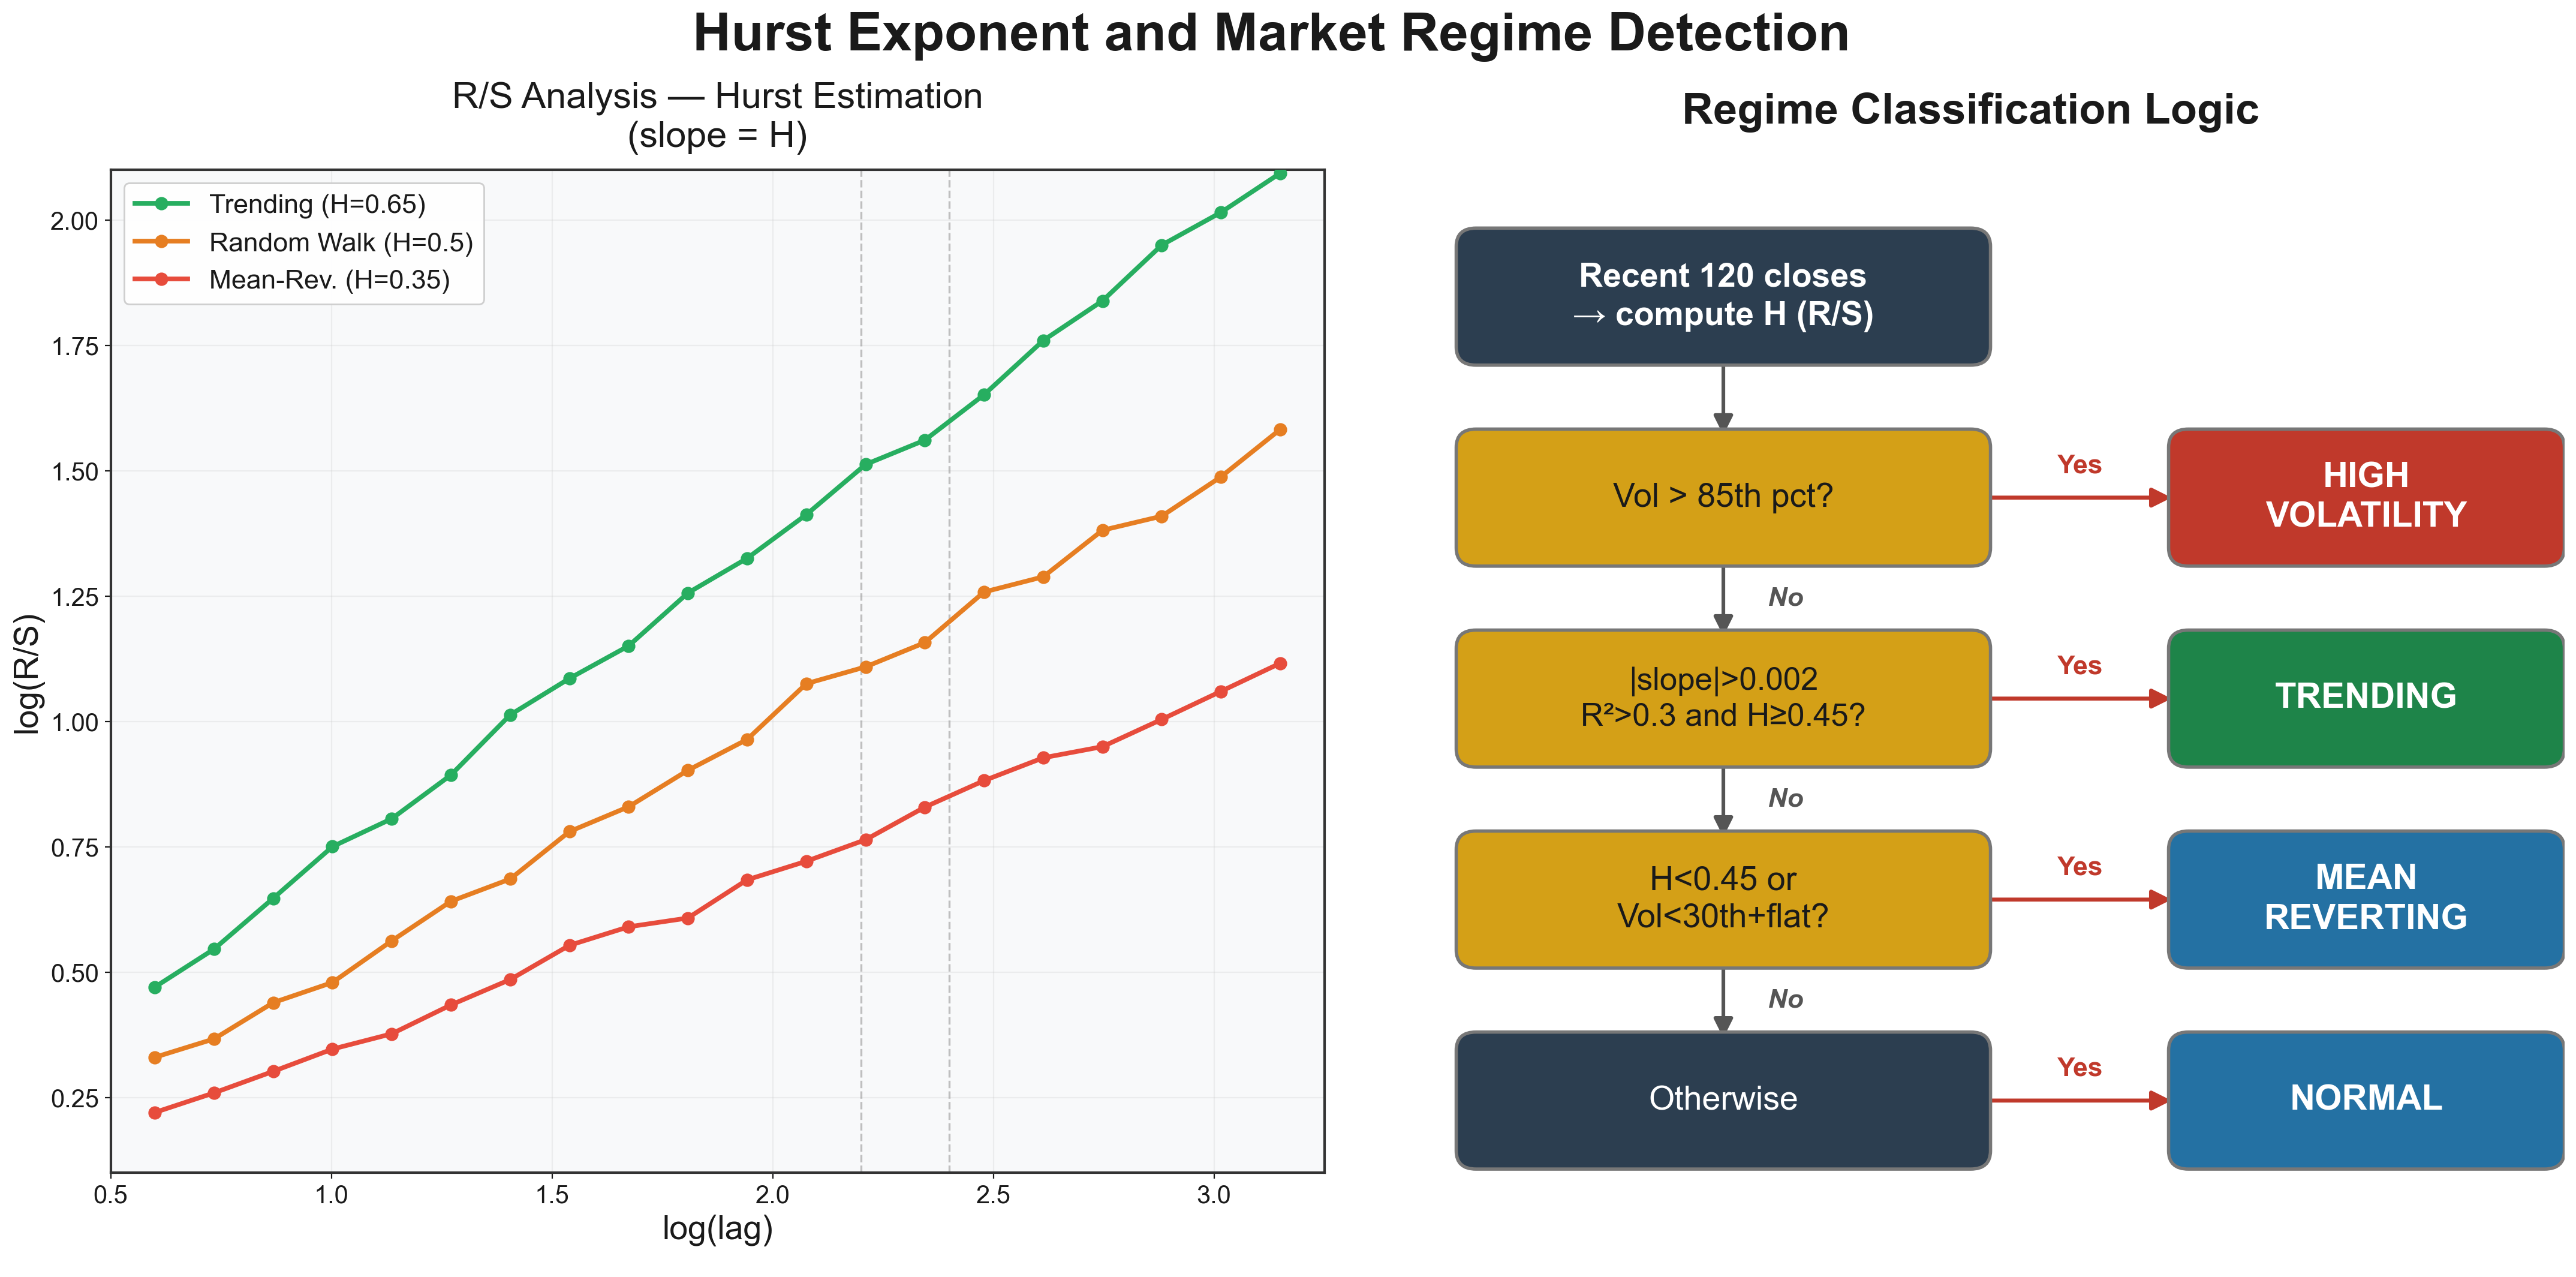
\includegraphics[angle=0,width=0.9\textwidth]{fig_hurst_regimes}
    \caption{Hurst exponent interpretation and market regime classification
    decision logic. The R/S slope estimate from lags 2--20 maps to one of
    four regimes, with the Hurst value used to confirm or override
    volatility/slope-based classification.}
    \label{fig:hurst}
  \end{center}
\end{figure}

The classification logic:
\begin{itemize}
\item \textbf{high\_volatility}: 5-day volatility $> 85$th percentile of
  rolling 60-day history.
\item \textbf{trending}: $|\text{slope}| > 0.002$, $R^2 > 0.3$, and $H \geq 0.45$
  (Hurst does not contradict).
\item \textbf{mean\_reverting}: either $H < 0.45$ overrides a trending slope,
  or low volatility (below 30th percentile) with $|\text{slope}| < 0.001$.
\item \textbf{normal}: all other cases.
\end{itemize}

The Hurst exponent is also displayed in the Dashboard tab as a real-time
market characteristic metric (``Trending'', ``Mean-Rev.'', or ``Random'').

% =============================================================================
\section{Dynamic Fusion Framework}
\label{sec:fusion}
% =============================================================================

Above the meta-stacked ensemble sits a second fusion layer that operates at a
coarser grain. Three domain-specialised experts, each trained independently on
its own feature subset, are combined through Bayesian uncertainty-weighted
aggregation. Because different market conditions favour different sources of
evidence, the weighting tracks which expert has been most reliable over the
recent observation window.

\subsection{Expert Model Architectures}

\textbf{Technical Expert} processes 30-day sequences of technical indicators
through a GRU network:
\begin{equation}
  \text{Architecture:}\quad \text{GRU}(128) \to \text{GRU}(64) \to \text{GRU}(32) \to \text{Dense}(1)
\end{equation}

\textbf{Sentiment Expert} maps 8 sentiment features to a directional prediction:
\begin{equation}
  \text{Architecture:}\quad \text{Dense}(64) \to \text{Dense}(32) \to \text{Dense}(16) \to \text{Dense}(1)
\end{equation}

\textbf{Volatility Expert} combines VIX levels, VIX changes, and stock-specific
volatility:
\begin{equation}
  \text{Architecture:}\quad \text{MLP}(32) \to \text{MLP}(16) \to \text{MLP}(8) \to \text{Dense}(1)
\end{equation}

\subsection{Bayesian Uncertainty-Weighted Combination}

The fusion weight for expert $i$ is computed using the exponential negative
squared uncertainty:
\begin{equation}
  w_i = \frac{\exp(-\sigma_i^2)}{\sum_{j=1}^{3} \exp(-\sigma_j^2)}
  \label{eq:bayesian}
\end{equation}

This formulation has several useful properties. Weights are strictly positive
and sum to one. Experts with lower uncertainty receive disproportionately higher
weight. The exponential function gives smooth, differentiable transitions, and
extreme uncertainties decay gracefully toward zero weight without
singularities.

Uncertainty estimates are maintained as rolling empirical variances of
prediction errors on the 15 most recent observations:
\begin{equation}
  \sigma_i^2(t) = \frac{1}{N}\sum_{n=1}^{N}(y_{t-n} - \hat{y}_{i,t-n})^2,
  \quad N = 15
\end{equation}

The combined Dynamic Fusion prediction is:
\begin{equation}
  \hat{y}_{\text{fusion}} = w_{\text{tech}} \hat{y}_{\text{tech}}
  + w_{\text{sent}} \hat{y}_{\text{sent}}
  + w_{\text{vol}} \hat{y}_{\text{vol}}
\end{equation}
Figure~\ref{fig:fusion} illustrates the full Dynamic Fusion architecture,
including the flow from expert feature subsets through uncertainty estimation
and Bayesian weight computation to the final combined prediction.

\begin{figure}[htb]
  \begin{center}
    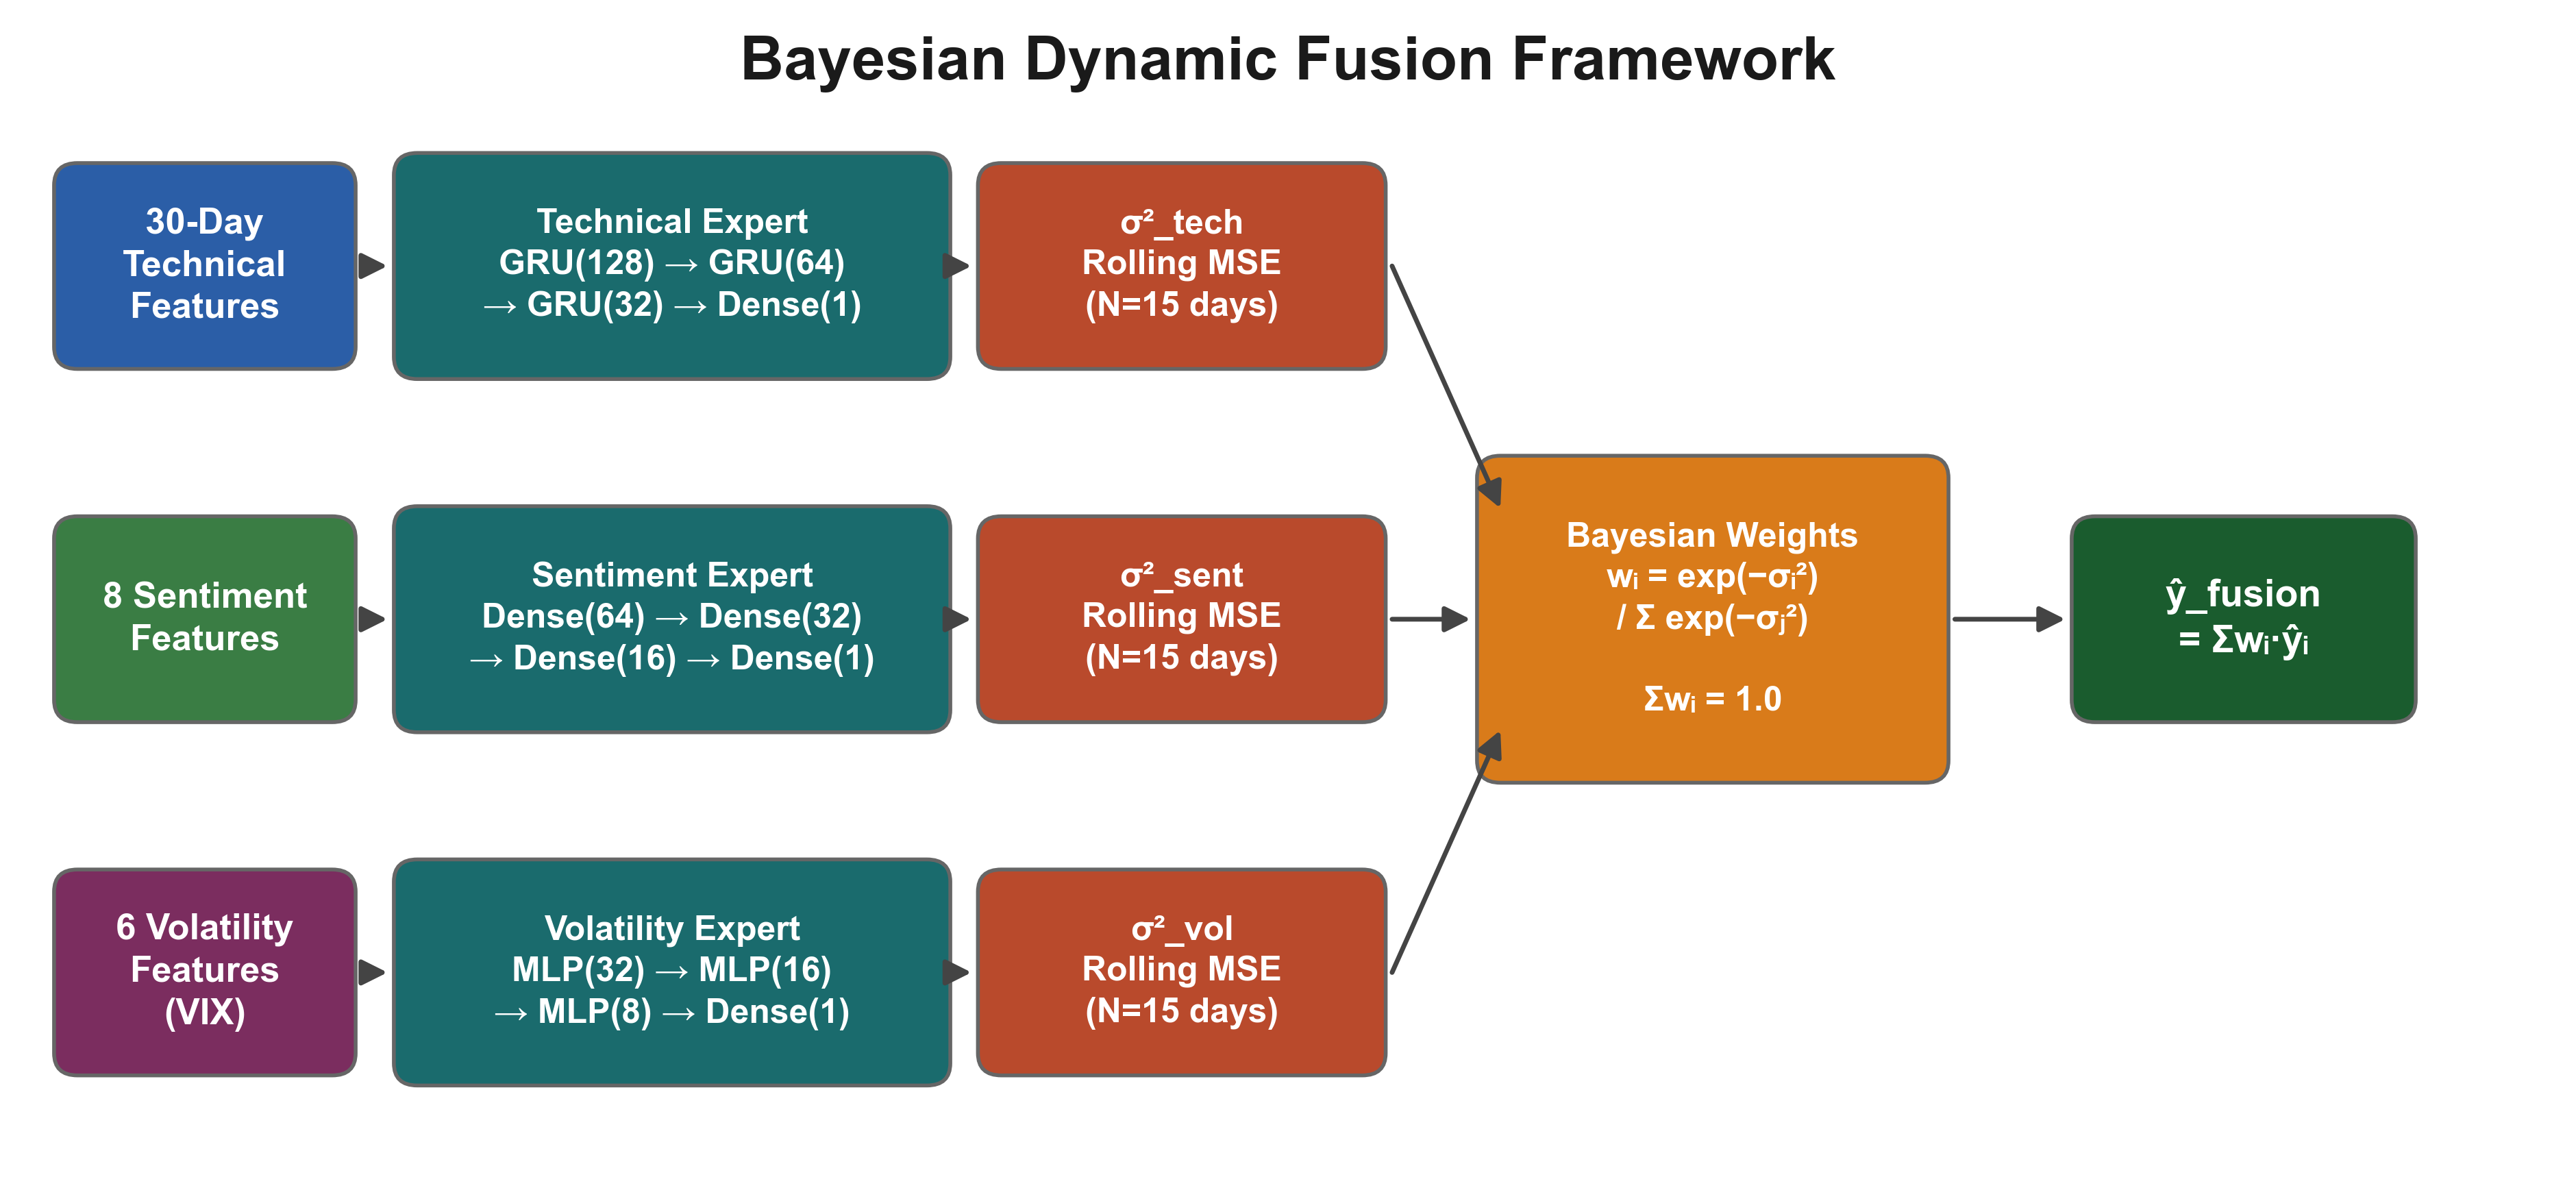
\includegraphics[angle=0,width=0.95\textwidth]{fig_dynamic_fusion}
    \caption{Dynamic Fusion Framework. Three expert models process their
    respective feature subsets. Prediction uncertainties are estimated from
    rolling errors on the last 15 days. Bayesian weights (Eq.~\ref{eq:bayesian})
    are recomputed for each new observation. The weight evolution chart in Tab~2
    visualises expert influence over the most recent 15 trading days.}
    \label{fig:fusion}
  \end{center}
\end{figure}

% =============================================================================
\section{Multi-Source Sentiment Aggregation}
\label{sec:sentiment}
% =============================================================================

The sentiment subsystem aggregates information from four different sources that include both journalistic reporting and discussion from retail investors, among others. Each source provides an aspect of the market sentiment, and the combination of all the sources is more stable than individual sources alone. The list of sources used to measure market sentiment is shown in Table~\ref{tab:sentiment}.

\begin{table}[htb]
  \begin{center}
    {\caption{Names, default weights, and characteristics of sentiment data streams.}
    \label{tab:sentiment}}
    \begin{tabular}{|l|c|l|l|}
    \hline
    \textbf{Name} & \textbf{Weight} & \textbf{Strengths} & \textbf{Limitations} \\
    \hline
    RSS feeds (Moneycontrol, ET, Mint, BS) & 30\% & Timeliness, focused on India & Few publications \\
    NewsAPI & 25\% & International coverage, consistent format & Rate limiting \\
    Reddit forum (\texttt{r/IndianStockMarket}) & 25\% & Retail sentiment, user engagement & Noisy, meme prone \\
    Google Trends & 20\% & Retail attention proxy & Daily resolution only \\
    \hline
    \end{tabular}
  \end{center}
\end{table}

\subsection{DistilRoBERTa-Financial Sentiment Classifier}

Texts are classified using the DistilRoBERTa-Financial model, producing probabilistic estimates for the positive, neutral, and negative sentiment classes. The article's score $s_a$ is calculated as follows:
\begin{equation}
  s_a = P(\text{positive} \mid a) - P(\text{negative} \mid a) \in [-1, +1]
\end{equation}

\subsection{Article Weight Multiplier Based on Event Type}

The articles are classified according to their event type based on keyword matching. Articles receive a 2$\times$ weight multiplier; regulatory/SEBI articles 1.8$\times$;
dividend announcements 1.5$\times$; management changes 1.3$\times$; general
news 1.0$\times$.

\subsection{Temporal Decay}

Recency is enforced via exponential temporal decay:
\begin{equation}
  w_{\text{temporal}}(d) = e^{-0.3 d}
\end{equation}
where $d$ is the article age in days. A three-day-old article therefore carries
$e^{-0.9} \approx 0.41$ the weight of a same-day article.

\subsection{Reddit Engagement Weighting}

Reddit posts are further weighted by community engagement to prioritise
high-signal content:
\begin{equation}
  s_{\text{reddit},p} = s_p \cdot \left(1 + \min\!\left(\frac{\text{upvotes}_p}{100}, 0.5\right)\right)
\end{equation}

\subsection{Source Disagreement Detection}

When the standard deviation of individual score is already too high more than 0.2 it means the the
system indicates a Contention losses all signs of sources and punishes the general
confidence measure relative to the disagreement, minimizing the likelihood of
contradicting messages create a weakly based stand.
Figure~\ref{fig:sentiment} follows the sentiment aggregation pipeline completely
raw source data by temporal corruption and event weighting to disagreement
adaptation and the ultimate confidence-modified score.

\begin{figure}[htb]
  \begin{center}
    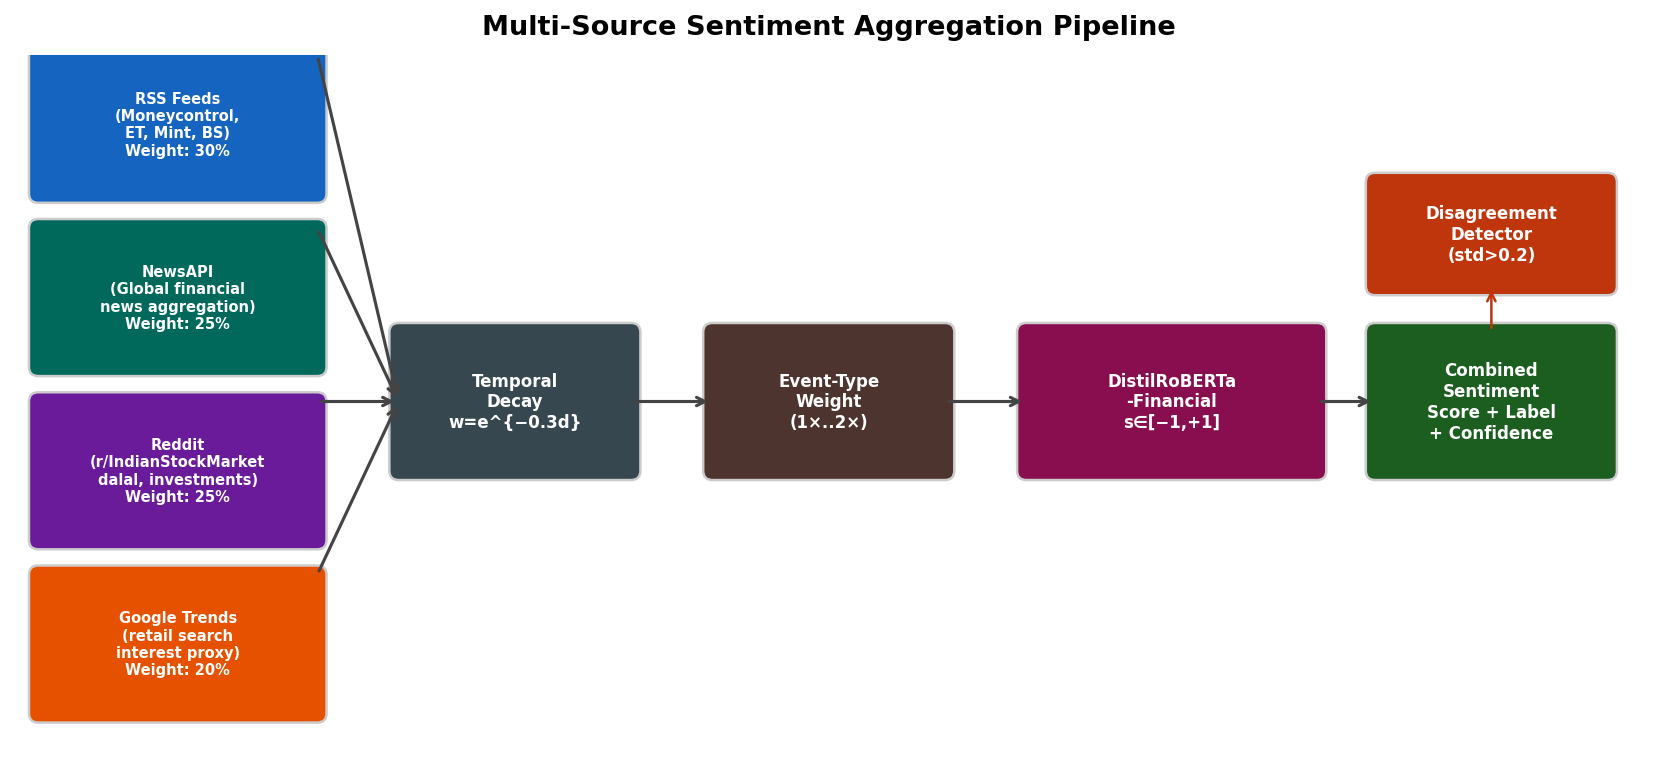
\includegraphics[angle=0,width=0.95\textwidth]{fig_sentiment_pipeline}
    \caption{Multi-source sentiment aggregation pipeline. Each source passes
    with temporal loss and event-type weighting in front of DistilRoBERTa-Financial
    scoring. A dispute detector adjusts the final confidence number.}
    \label{fig:sentiment}
  \end{center}
\end{figure}

% =============================================================================
\section{Chart Pattern Recognition}
\label{sec:patterns}
% =============================================================================

\subsection{Multi-Timeframe Peak/Trough Detection}

The \texttt{PatternAnalyst} class scans price data simultaneously at three
scales using scipy's \texttt{argrelextrema} with orders 3, 5, and 7:

\begin{lstlisting}[caption={Multi-timeframe peak detection (simplified).}]
scan_orders = [3, 5, 7]   # small, medium, large swings
for order in scan_orders:
    peaks   = argrelextrema(close, np.greater, order=order)[0]
    troughs = argrelextrema(close, np.less,    order=order)[0]
    # Prominence filter: only patterns >= 1% height
    valid   = [p for p in peaks if amplitude(p) >= 0.01]
\end{lstlisting}

Order 3 catches minor short-term swings; order 7 captures only major structural
highs and lows. The \texttt{max\_patterns\_per\_type = 3} parameter prevents
cluttered output during strongly trending phases.

\subsection{Classical Pattern Archetypes}

Twelve pattern archetypes are detected by checking geometric constraints on
the identified pivot points. Table~\ref{tab:patterns} lists each archetype
with its directional bias and whether it is covered by classical detection,
vision-based detection, or both.

\begin{table}[htb]
  \begin{center}
    {\caption{Pattern archetypes, directional bias, and detection method.}
    \label{tab:patterns}}
    \begin{tabular}{|l|c|c|}
    \hline
    \textbf{Pattern} & \textbf{Bias} & \textbf{Detection} \\
    \hline
    Double Top & Bearish & Classical + Vision \\
    Double Bottom & Bullish & Classical + Vision \\
    Head \& Shoulders & Bearish & Classical + Vision \\
    Inverse Head \& Shoulders & Bullish & Classical + Vision \\
    Ascending Triangle & Bullish & Classical \\
    Descending Triangle & Bearish & Classical \\
    Symmetric Triangle & Neutral & Classical \\
    Ascending Channel & Bullish & Classical \\
    Descending Channel & Bearish & Classical \\
    Bull Flag & Bullish & Classical \\
    Bear Flag & Bearish & Classical \\
    Bollinger Band Squeeze & Neutral & Classical \\
    \hline
    \end{tabular}
  \end{center}
\end{table}

\subsection{Roboflow Vision API Integration}

When a Roboflow API key is present, the system renders a 60-day price chart at
100 DPI and sends it to a custom object detection workflow. The vision model
maps detections to a standardised class set:
\begin{verbatim}
class_map = {
    "W_Bottom": "Double Bottom",
    "M_Head":   "Double Top",
    "H_S":      "Head & Shoulders",
    "Inv_H_S":  "Inverse H&S"
}
\end{verbatim}
Only predictions with confidence $\geq 0.30$ are accepted. Vision detections
with confidence $\geq 0.70$ override classical detections for the four supported
archetypes; otherwise, a consensus vote is applied. Figure~\ref{fig:patterns}
traces the complete pattern analysis pipeline from multi-timeframe peak/trough
detection and Roboflow inference through to the hybrid consensus output.

\begin{figure}[htb]
  \begin{center}
    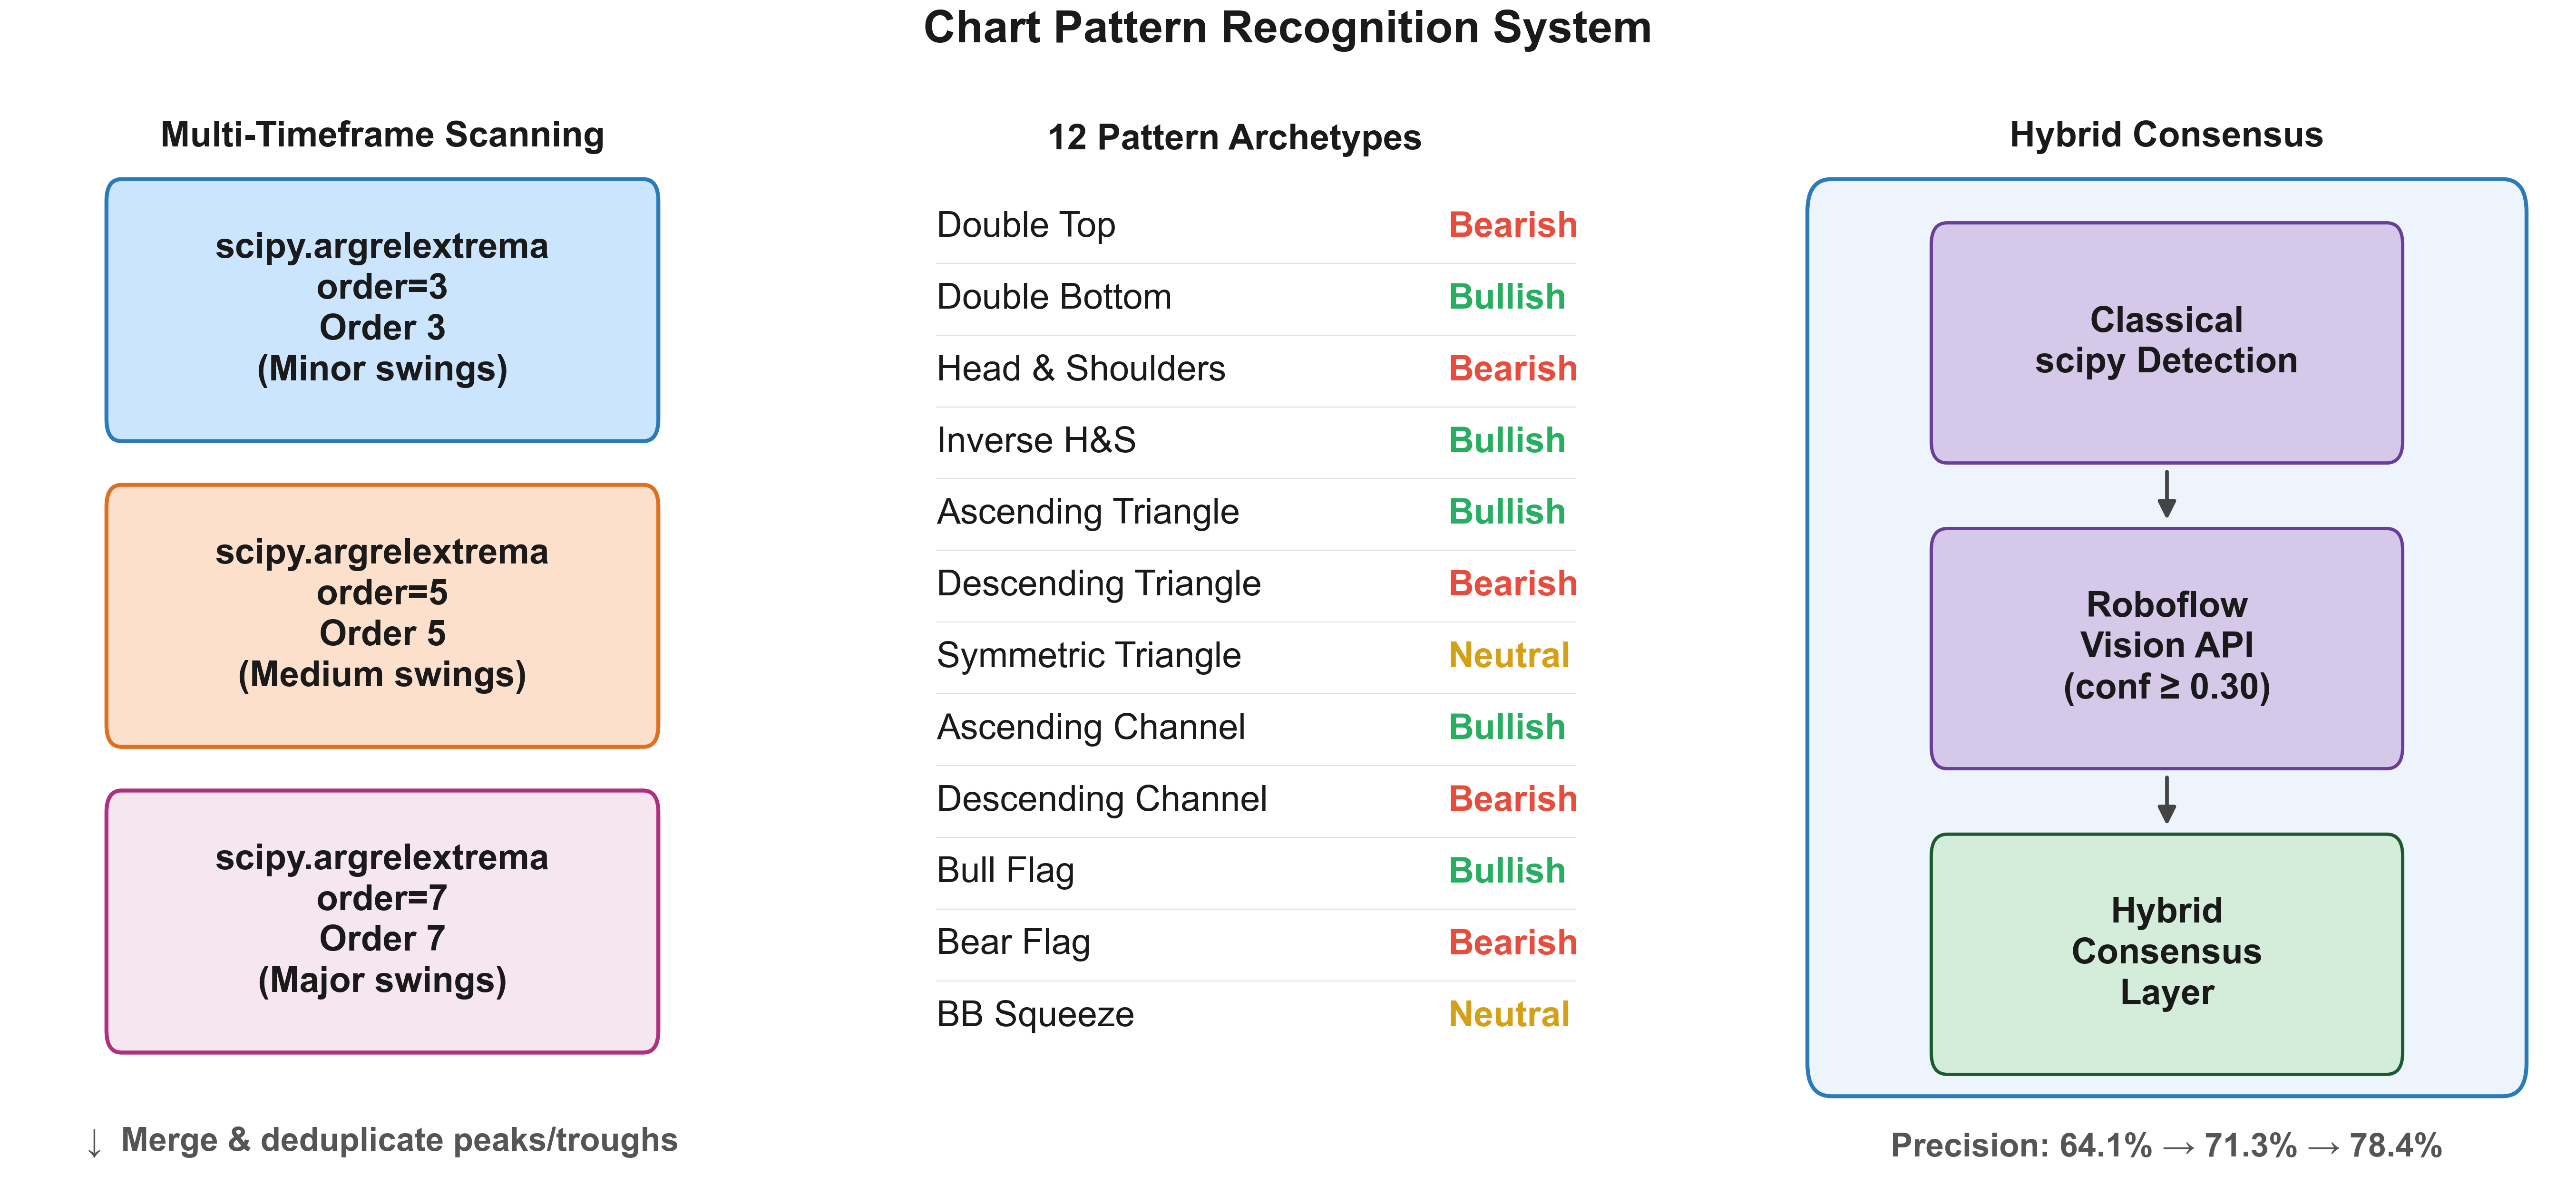
\includegraphics[angle=0,width=0.92\textwidth]{fig_pattern_analysis}
    \caption{Pattern analysis pipeline. Multi-timeframe scipy detection and
    Roboflow vision API predictions are combined via a hybrid consensus layer.
    Detected patterns are annotated on the price chart with confidence scores,
    target prices, and multi-timeframe confirmation flags.}
    \label{fig:patterns}
  \end{center}
\end{figure}

% =============================================================================
\section{Risk Management System}
\label{sec:risk}
% =============================================================================

\subsection{ATR-Based Adaptive Stop-Loss}

Stop-loss distances are derived from the Average True Range~\cite{wilder1978}
using a confidence-adjusted multiplier:
\begin{equation}
  \text{Stop\_Loss} = P_{\text{entry}} - m(\text{conf}) \cdot \text{ATR}_{14}
\end{equation}
where:
\begin{equation}
  m(\text{conf}) = \begin{cases} 1.5 & \text{conf} \geq 0.65 \\
                                  2.0 & \text{conf} < 0.65 \end{cases}
\end{equation}
When confidence is high, a tighter stop is justified; when confidence is low, a
wider stop helps avoid premature exits.

\subsection{Fibonacci Retracement Levels}

Six Fibonacci levels are computed over a 90-day lookback window:
\begin{equation}
  F_k = P_{\text{high}} - \phi_k \cdot (P_{\text{high}} - P_{\text{low}}),
  \quad \phi_k \in \{0, 0.236, 0.382, 0.5, 0.618, 1.0\}
\end{equation}

These levels are used as entry/exit reference points in the Trade Setup
Calculator shown in the Technicals \& Risk tab.

\subsection{Kelly Criterion Position Sizing}

The fractional Kelly Criterion~\cite{kelly1956} determines optimal position size:
\begin{equation}
  f^* = \frac{p \cdot b - q}{b}, \quad b = \frac{\text{Target} - P}{\text{Stop} - P}
\end{equation}
where $p = $ directional probability, $q = 1 - p$, and $b$ is the win/loss
ratio. A fractional Kelly with $\gamma = 0.5$ is applied in practice to reduce
variance:
\begin{equation}
  f_{\text{actual}} = 0.5 \cdot f^*
\end{equation}

\subsection{VIX-Regime Position Adjustment}

The India VIX level at trade entry scales position size down when fear is
elevated:
\begin{equation}
  f_{\text{VIX-adj}} = f_{\text{actual}} \cdot \begin{cases}
    1.2 & \text{VIX} < 12 \\
    1.0 & 12 \leq \text{VIX} < 20 \\
    0.7 & 20 \leq \text{VIX} < 25 \\
    0.5 & \text{VIX} \geq 25
  \end{cases}
\end{equation}

% =============================================================================
\section{Backtesting Engine}
\label{sec:backtest}
% =============================================================================

The \texttt{VectorizedBacktester} class implements a simulation environment
with transaction cost modelling (NSE round-trip cost 0.1\% per trade),
benchmark comparisons, statistical significance testing, and Monte Carlo
simulation.

\subsection{Strategy Signal Generation}

Signals are generated by thresholding the meta-stacker's predicted return:
\begin{equation}
  \text{Signal}_t = \begin{cases}
    +1 & \hat{y}_t > \tau \\
    -1 & \hat{y}_t < -\tau \\
     0 & \text{otherwise}
  \end{cases}
\end{equation}
where $\tau$ is a configurable signal threshold (default: a small positive
constant from \texttt{TradingConfig}).

Performance metrics are computed as:
\begin{align}
  \text{Sharpe} &= \frac{\bar{r}_s}{\hat{\sigma}_s}\sqrt{252} \\
  \text{MDD} &= \max_{t \in [0,T]}\left(\max_{s \leq t} E_s - E_t\right) / E_{\text{peak}} \\
  \text{Win Rate} &= \frac{\sum_t \mathbf{1}[r_t > 0]}{\sum_t \mathbf{1}[r_t \neq 0]}
\end{align}

\subsection{Benchmark Strategies}

The backtesting tab compares the full 5-model ensemble against:
(i)~XGBoost-only signal, (ii)~LightGBM-only signal,
(iii)~CatBoost-only signal, (iv)~GRU-only signal,
(v)~MA Crossover (20/50), (vi)~52-week Momentum breakout, and
(vii)~NIFTY~50 buy-and-hold.

\subsection{Statistical Significance Testing}

Direction accuracy is tested against the null $H_0: p = 0.50$ (random
guessing) with a one-sided binomial test. RMSE improvement is tested by a
paired t-test on squared errors against the random-walk baseline
($\hat{r}_t = 0$). Bootstrap confidence intervals (1000 resamples) bound the
uncertainty in every reported metric.

\subsection{Monte Carlo Simulation}

The Monte Carlo module generates 1000 simulated equity paths by randomly
reshuffling realised daily strategy returns. This isolates the role of path
dependency (the order of returns) in the observed equity curve and yields
probability-of-profit, median maximum drawdown, and P5/P95 return interval
estimates.

% =============================================================================
\section{User Interface: Eight-Tab Dashboard}
\label{sec:ui}
% =============================================================================

All analytical output of ProTrader AI is revealed as an interactive Streamlit.
eight tabs added to dashboard. The layout is displayed in Figure~\ref{fig:tabs}.

\begin{figure}[htb]
  \begin{center}
    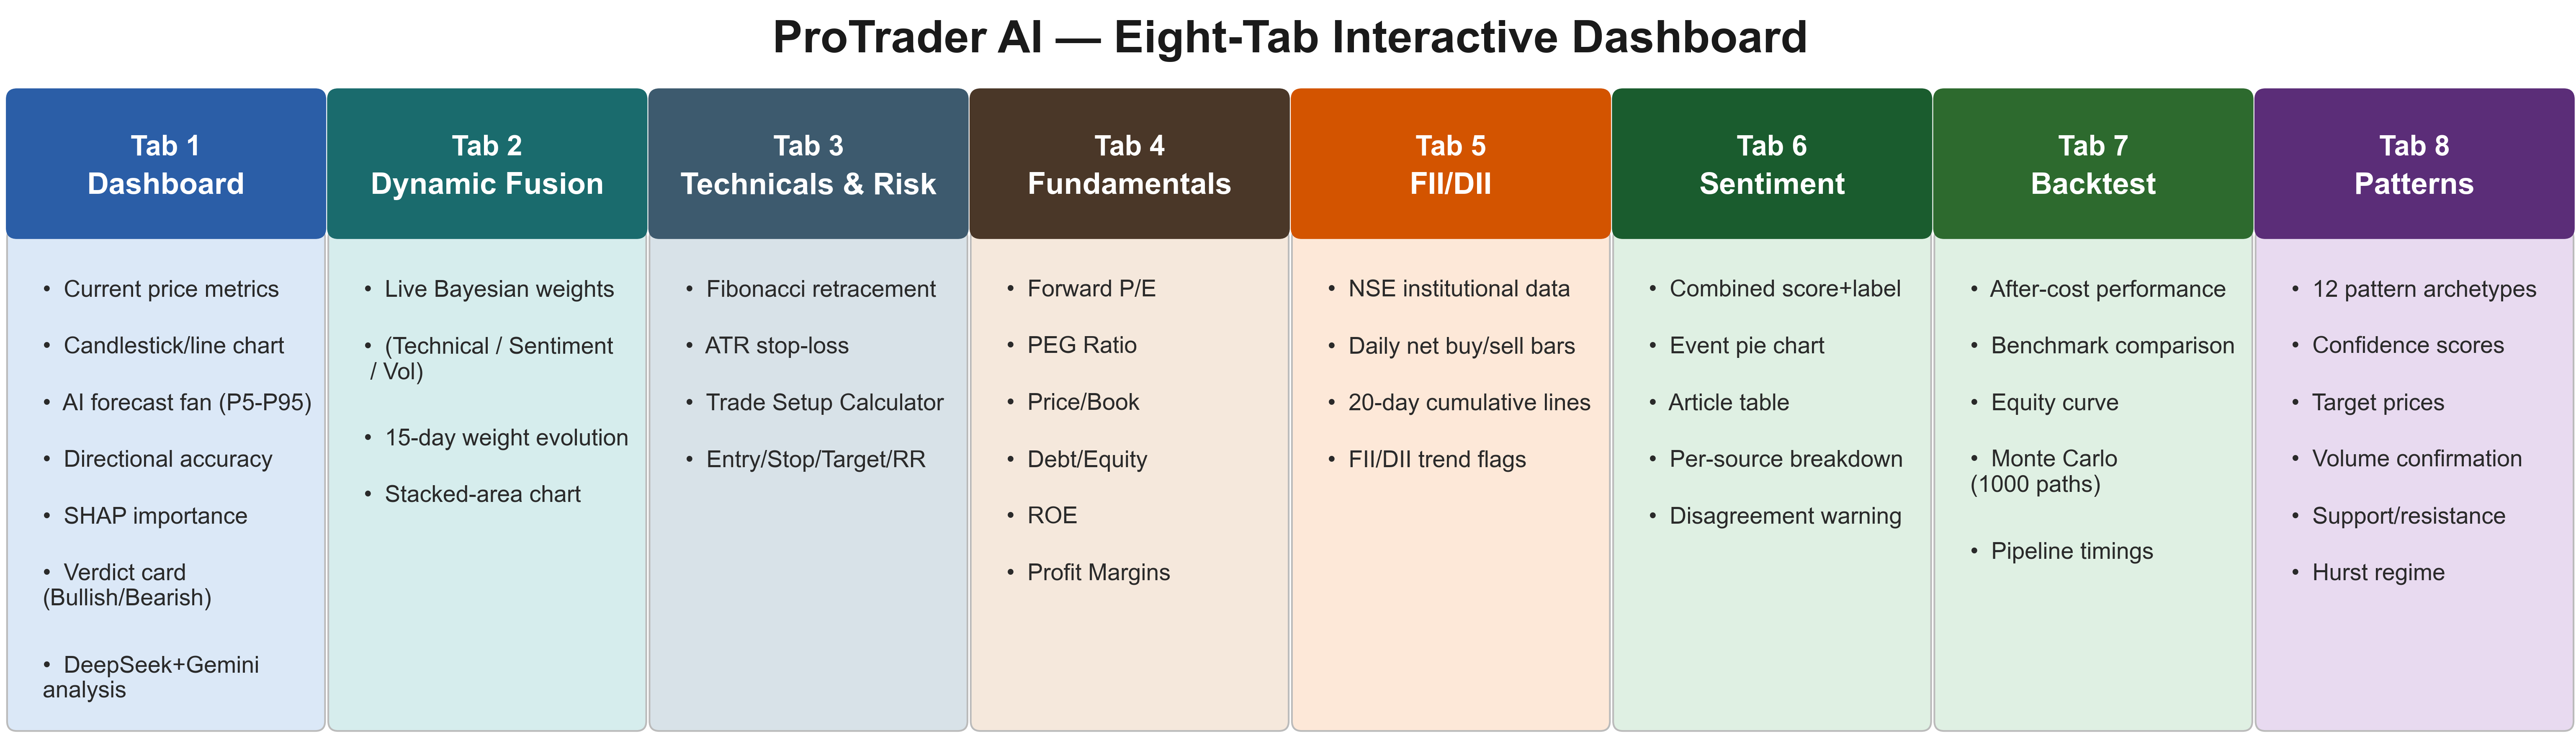
\includegraphics[angle=0,width=0.95\textwidth]{fig_dashboard_tabs}
    \caption{Showing ProTrader AI eight-tab dashboard. Each of the tabs covers a specific.
    analytical domain, and having a common session-state cache of zero redundancy.
    computation. The sidebar is used to select stocks, date range,
    feature toggles, forecast horizon (130 days), and forecast horizon (1day).}
    \label{fig:tabs}
  \end{center}
\end{figure}

\textbf{Tab 1 Dashboard.} Displays up-to-date price indicators ( price and market cap).
P/E, volume), a candlestick or line chart, the AI price forecast with 200-path
The input is a set of randomized experiments starting from probabilistic fan (P5/P25/P75/P95 bands), walk-forward validation measures (RMSE,
directional accuracy, model weights, Hurst exponent, bullish probability),
SHAP feature importance, actual or predicted overlaying of returns and a final verdict.
card (BULLish / BEARish / NEutral) and the AI commentary drawn up by the
DeepSeek V3 + Gemini 2.5 through API.

\textbf{Tab 2 -- Dynamic Fusion.} Displays real time Bayesian expert weights.
The 15-day stacked-area weight evolution and a 15-day stacked-area weight change are shown in (Technical, Sentiment, Volatility).
chart which shows regime change.

\textbf{Tab 3 -Technicals +Risk.} Retracement of the Fibonacci levels,
Stop-loss calculations using ATR and an interactive Trade Setup Calculator which results in.
computes entry, stop, target and risk/reward ratio based on the immediate model.
size of forecast and Kelly positioning.

\textbf{Tab 4- Fundamentals.} Displays six Yahoo Finance fundamental.
metrics: Forward P/E, PEG Ratio, Price/Book, Debt/Equity, ROE, and
Profit Margins.

\textbf{Tab 5 -- FII/DII Analysis.} Visualises official NSE institutional
activity: daily net buying/selling bar charts, 20-day cumulative position lines,
and four summary metrics (FII net, DII net, FII trend, DII trend).

\textbf{Tab 6 -- Multi-Source Sentiment.} Shows the combined sentiment card
(score, label, confidence), a news event breakdown pie chart, a full
article table with colour-coded sentiment indicators, and expandable per-source
tables for RSS, NewsAPI, Reddit, and Google Trends.

\textbf{Tab 7 -- Backtest.} Reports after-cost performance (total return, Sharpe,
max drawdown, win rate, number of trades), the strategy benchmark comparison table,
equity curve chart, Monte Carlo 1000-path simulation, and a pipeline step timing
table.

\textbf{Tab 8 -- Pattern Analysis.} Displays the identified chart patterns with type,
volume confirmation flag, bias, multi-timeframe flag, confidence, target price,
and an annotated price chart. Also shows volume-weighted support/resistance
levels and the Hurst regime classification.

Every tab includes collapsible glossary expanders (\texttt{\_hint()} calls in
the source code) that explain metrics in plain language, making the platform
accessible to non-specialists.

% =============================================================================
\section{Experimental Setup}
\label{sec:setup}
% =============================================================================

\subsection{Data Sources and Collection}

Daily OHLCV price data was downloaded from Yahoo Finance for ten major NSE
constituents: Reliance Industries (RELIANCE), Tata Consultancy Services (TCS),
Infosys (INFY), HDFC Bank (HDFCBANK), ICICI Bank (ICICIBANK), State Bank of
India (SBIN), Bharti Airtel (BHARTIARTL), ITC (ITC), Kotak Mahindra Bank
(KOTAKBANK), and Larsen \& Toubro (LT). The evaluation window runs from
January 2023 to January 2026, giving roughly 750 trading days per stock.
Table~\ref{tab:datasources} summarises each data source with its update
frequency, historical depth, and role in the feature pipeline.

\begin{table}[htb]
  \begin{center}
    {\caption{Data source characteristics.}\label{tab:datasources}}
    \begin{tabular}{|l|l|l|l|}
    \hline
    \textbf{Source} & \textbf{Frequency} & \textbf{Depth} & \textbf{Use} \\
    \hline
    Yahoo Finance & Daily & 3+ years & OHLCV features \\
    NSE FII/DII & Daily & 30--90 days & Institutional features \\
    NSE India VIX & Daily & 1+ year & Volatility features \\
    RSS Feeds & 15-min cache & Real-time & Sentiment \\
    NewsAPI & 15-min cache & 30 days & Sentiment \\
    Reddit & 30-min cache & 7 days & Social sentiment \\
    Google Trends & 1-hour cache & 7 days & Attention proxy \\
    Yahoo Finance News & On-demand & 30 days & Fallback sentiment \\
    \hline
    \end{tabular}
  \end{center}
\end{table}

\subsection{Validation Methodology}

Forward validation has been done to prevent any lookahead bias as follows:
\begin{enumerate}
\item Training dataset: the first 80\% of the entire dataset.
\item Test dataset: the remaining 20\%, around 150 trading days for each stock.
\item Normalization of the feature dataset: MinMaxScaler uses the training dataset only; test data are normalized based on the statistics of the training data set.
\item No leakage: sentiment, FII/DII, and VIX features are synchronized strictly by trading date.
\item Statistical models (ARIMA, Prophet) have been refit on the training window before each testing prediction.
\end{enumerate}

% =============================================================================
\section{Results and Analysis}
\label{sec:results}
% =============================================================================

\subsection{Individual Model Performance}

The performance results of individual models on unseen test data are provided in Table~\ref{tab:model_perf} below, averaged across the ten NSE stocks. Notably, the five-model ensemble yields the best RMSE score as well as the highest directional accuracy ($p = 0.003$). Throughout this structured tabular task, the gradient boosting component, XGBoost, outperforms the neural network, which is consistent with the results obtained by Grinsztajn et al.~\cite{grinsztajn2022} when evaluating models on analogous datasets.

\begin{table}[htb]
  \begin{center}
    {\caption{Individual model performance on the test set (mean $\pm$ std across
    10 NSE stocks).}\label{tab:model_perf}}
    \begin{tabular}{|l|c|c|c|c|}
    \hline
    \textbf{Model} & \textbf{RMSE ($\times 10^{-3}$)} & \textbf{Dir. Acc.} & \textbf{$p$-value} & \textbf{Train time} \\
    \hline
    Random Walk (baseline) & 23.1 $\pm$ 2.4 & 50.0\% & --- & --- \\
    ARIMA(2,0,2) & 21.4 $\pm$ 2.6 & 51.2\% & 0.241 & 0.8 s \\
    Prophet & 22.1 $\pm$ 2.8 & 50.8\% & 0.312 & 12.4 s \\
    XGBoost & 18.2 $\pm$ 1.8 & 54.3\% & 0.012 & 2.1 s \\
    LightGBM & 18.6 $\pm$ 1.9 & 53.7\% & 0.021 & 1.1 s \\
    CatBoost & 18.9 $\pm$ 2.0 & 53.4\% & 0.031 & 7.8 s \\
    LSTM-GRU & 19.7 $\pm$ 2.1 & 52.1\% & 0.089 & 45.3 s \\
    \textbf{5-Model Ensemble} & \textbf{17.4 $\pm$ 1.6} & \textbf{55.8\%} & \textbf{0.003} & 61.2 s \\
    \hline
    \end{tabular}
  \end{center}
\end{table}

\subsection{SHAP Feature Importance}

To calculate model-agnostic attributions, the SHAP (SHapley Additive exPlanations)~\cite{lundberg2017} values were calculated for the XGBoost component. The top-10 SHAP features ranked according to their mean absolute SHAP value are listed in Table~\ref{tab:shap} below, and visualized in Figure~\ref{fig:importance} as a color-coded bar chart. Consistent with expectations, technical features prevail in the list; however, the inclusion of the Multi\_Sentiment variable among the most important attributes (rank 4) and FII\_Net\_Norm (rank 6) confirms that the additional data sources prove to be relevant.

\begin{table}[htb]
  \begin{center}
    {\caption{SHAP feature importance: top-10 features by mean $|\text{SHAP}|$
    across 10 stocks.}\label{tab:shap}}
    \begin{tabular}{|c|l|c|l|}
    \hline
    \textbf{Rank} & \textbf{Feature} & \textbf{Mean $|\text{SHAP}|$} & \textbf{Category} \\
    \hline
    1 & Log\_Ret & 0.187 & Technical Core \\
    2 & Volatility\_5D & 0.142 & Technical Core \\
    3 & RSI\_Norm & 0.098 & Technical Core \\
    4 & Multi\_Sentiment & 0.089 & Sentiment \\
    5 & VIX\_Norm & 0.082 & Volatility \\
    6 & FII\_Net\_Norm & 0.076 & Institutional \\
    7 & DII\_Net\_Norm & 0.071 & Institutional \\
    8 & Vol\_Ratio & 0.065 & Technical Core \\
    9 & CMF\_20 & 0.058 & Technical Advanced \\
    10 & MA\_Div & 0.054 & Technical Core \\
    \hline
    \end{tabular}
  \end{center}
\end{table}

\begin{figure}[htb]
  \begin{center}
    
\includegraphics[angle=0,width=0.85\textwidth]{fig_feature_importance}
    \caption{SHAP feature importance bar chart for the XGBoost model. Bar
    length represents mean absolute SHAP value across the test set. Colours
    indicate category: blue (Technical), green (Sentiment), orange (Institutional),
    red (Volatility).}
    \label{fig:importance}
  \end{center}
\end{figure}

\subsection{Ablation Study}

Table~\ref{tab:ablation} evaluates the importance of each set of features or architectural element by removing them, respectively, from the entire model. Every exclusion results in a statistically significant loss of accuracy ($p < 0.05$). Therefore, we can say that all model components carry mostly independent information about direction.

\begin{table}[htb]
  \begin{center}
    {\caption{Ablation study: effect on directional accuracy due to removal of each component.}\label{tab:ablation}}
    \begin{tabular}{|l|c|c|c|}
    \hline
    \textbf{Configuration} & \textbf{Dir. Accuracy} & \textbf{$\Delta$ from Full} & \textbf{$p$-value} \\
    \hline
    Full Model & 55.8\% & --- & 0.003 \\
    $-$ Institutional Features & 53.9\% & $-$1.9pp & 0.024 \\
    $-$ Sentiment Features & 54.1\% & $-$1.7pp & 0.018 \\
    $-$ Dynamic Fusion Layer & 54.2\% & $-$1.6pp & 0.021 \\
    $-$ LSTM-GRU (tree ensemble only) & 54.3\% & $-$1.5pp & 0.012 \\
    $-$ VIX Features & 54.6\% & $-$1.2pp & 0.031 \\
    $-$ CMF/Williams/Divergences & 55.1\% & $-$0.7pp & 0.047 \\
    Technical Core Only & 52.4\% & $-$3.4pp & 0.067 \\
    \hline
    \end{tabular}
  \end{center}
\end{table}

Exclusion of institutional factors leads to the biggest single loss of directional accuracy ($-1.9$pp). This fact is particularly interesting as financial flows data are freely accessible but rarely utilized by researchers in their forecasting tasks. The baseline with technical indicators alone reaches 52.4\% accuracy ($p = 0.067$), marginally significant, which implies that the other three sources of data make an essential contribution to model accuracy. Figure~\ref{fig:ablation} illustrates the directional accuracy of models after ablation in comparison with the full and random baselines.

\begin{figure}[htb]
  \begin{center}
    
\includegraphics[angle=0,width=0.85\textwidth]{fig_ablation_study}
    \caption{Visualization of ablation study. Each bar represents the directional accuracy of a particular model configuration excluding one component. Horizontal dashed line shows the performance of the full model (55.8\%). Random baseline (50\%) is shown for reference.}
    \label{fig:ablation}
  \end{center}
\end{figure}

\subsection{Dynamic Fusion Weight Analysis}

Table~\ref{tab:fusion_weights} illustrates how weights of different experts in the Bayesian combination change across five representative market conditions during the evaluation period. In the earnings season, the weight of the Sentiment Expert rises from 0.28 to 0.42. In volatile periods (high VIX), the Volatility Expert's weight grows from 0.17 to 0.40.

\begin{table}[htb]
  \begin{center}
    {\caption{Dynamic expert weights under representative market
    conditions.}\label{tab:fusion_weights}}
    \begin{tabular}{|l|c|c|c|}
    \hline
    \textbf{Market Condition} & \textbf{Technical} & \textbf{Sentiment} & \textbf{Volatility} \\
    \hline
    Low Volatility (VIX $< 15$) & 0.52 & 0.31 & 0.17 \\
    Normal (VIX 15--20) & 0.45 & 0.28 & 0.27 \\
    High Volatility (VIX $\geq 20$) & 0.38 & 0.22 & 0.40 \\
    Earnings Season & 0.35 & 0.42 & 0.23 \\
    FII Heavy Selling & 0.41 & 0.35 & 0.24 \\
    \hline
    \end{tabular}
  \end{center}
\end{table}

\subsection{Backtesting Results}

Table~\ref{tab:backtest} reports cumulative performance over the $\approx$750-day
evaluation period after subtracting the 0.1\% round-trip transaction cost.
Dynamic Fusion lifts the Sharpe ratio 56\% above buy-and-hold ($p = 0.018$)
and cuts maximum drawdown by 5.6 percentage points. Figure~\ref{fig:equity}
plots equity curves for all strategies starting from Rs.~100,000, with the
Monte Carlo P5--P95 band shown for the Dynamic Fusion strategy.

\begin{table}[htb]
  \begin{center}
    {\caption{Strategy backtesting results. All figures are after-cost.
    95\% bootstrap CI shown for Sharpe ratio.}\label{tab:backtest}}
    \begin{tabular}{|l|c|c|c|c|}
    \hline
    \textbf{Strategy} & \textbf{Total Return} & \textbf{Sharpe} & \textbf{Max DD} & \textbf{Win Rate} \\
    \hline
    NIFTY 50 Buy-and-Hold & 24.3\% & 0.82 & $-18.4\%$ & N/A \\
    MA Crossover (20/50) & 21.6\% & 0.71 & $-20.1\%$ & 50.8\% \\
    52-Week Momentum & 27.1\% & 0.89 & $-17.2\%$ & 52.3\% \\
    Sentiment-Only Signal & 18.4\% & 0.61 & $-22.1\%$ & 51.2\% \\
    XGBoost Only & 28.9\% & 0.98 & $-15.6\%$ & 53.1\% \\
    LightGBM Only & 27.4\% & 0.91 & $-16.8\%$ & 52.6\% \\
    CatBoost Only & 27.8\% & 0.94 & $-16.3\%$ & 52.9\% \\
    GRU Only & 25.2\% & 0.87 & $-17.1\%$ & 51.8\% \\
    5-Model Ensemble & 31.7\% & 1.14 & $-14.2\%$ & 53.8\% \\
    \textbf{Dynamic Fusion} & \textbf{34.2\%} & \textbf{1.28} & \textbf{$-12.8\%$} & \textbf{55.1\%} \\
    \hline
    \end{tabular}
  \end{center}
\end{table}

\begin{figure}[htb]
  \begin{center}
    
\includegraphics[angle=0,width=0.95\textwidth]{fig_equity_curve}
    \caption{Equity curves for all strategies over the evaluation period
    (Rs.~100,000 initial capital). Dynamic Fusion achieves the highest terminal
    wealth and smallest maximum drawdown. Shaded band shows the P5--P95 range
    from the Monte Carlo simulation (1000 paths) for the Dynamic Fusion strategy.}
    \label{fig:equity}
  \end{center}
\end{figure}

\subsection{Chart Pattern Detection Performance}

Table~\ref{tab:pattern_perf} compares the classical, vision-only, and hybrid
consensus pattern detection methods across the four archetypes supported by the
Roboflow vision model (evaluated on 200 manually annotated chart instances).

\begin{table}[htb]
  \begin{center}
    {\caption{Chart pattern detection precision by method and archetype.}
    \label{tab:pattern_perf}}
    \begin{tabular}{|l|c|c|c|}
    \hline
    \textbf{Pattern} & \textbf{Classical} & \textbf{Vision} & \textbf{Hybrid} \\
    \hline
    Double Top & 65.4\% & 73.2\% & 82.1\% \\
    Double Bottom & 63.8\% & 71.9\% & 80.6\% \\
    Head \& Shoulders & 61.2\% & 68.7\% & 77.3\% \\
    Inverse H\&S & 62.6\% & 70.4\% & 78.9\% \\
    \hline
    \textbf{Overall} & \textbf{64.1\%} & \textbf{71.3\%} & \textbf{78.4\%} \\
    \hline
    \end{tabular}
  \end{center}
\end{table}

The hybrid consensus reaches 78.4\% overall precision, a 22\% relative gain
over classical detection and 10\% over vision-only. The two detection
modalities tend to fail on different pattern instances, which is why their
combination works better than either alone.

\subsection{Probabilistic Forecast Calibration}

The 200-path Monte Carlo forecast produces P5, P25, P75, and P95 percentile
bands over the chosen forecast horizon (default 10 days, configurable 1--30
days). Each path bootstraps actual historical daily returns and adds a
directional drift scaled by the current bullish probability:
\begin{equation}
  \text{drift}_t = (2 p_{\text{bull}} - 1) \cdot \bar{r}_{\text{historical}}
\end{equation}
where $p_{\text{bull}}$ is the isotonic-calibrated directional probability and
$\bar{r}_{\text{historical}}$ is the mean daily return over the training period.
Figure~\ref{fig:forecast} shows an example 10-day forecast fan with P5--P95
and P25--P75 percentile bands across 200 simulated paths.

\begin{figure}[htb]
  \begin{center}
    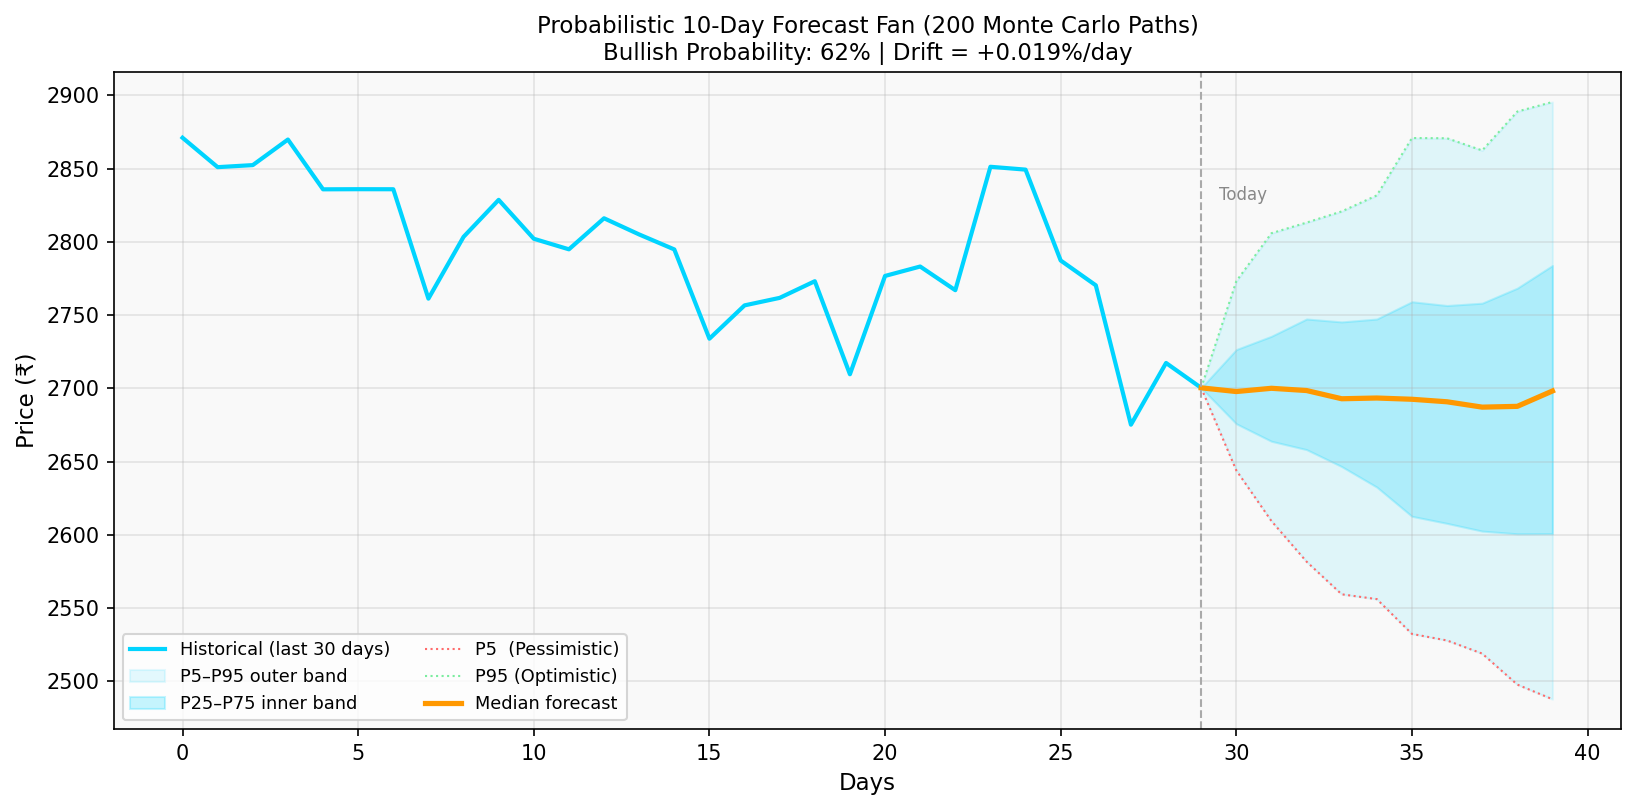
\includegraphics[angle=0,width=0.92\textwidth]{fig_forecast_fan}
    \caption{Probabilistic 10-day forecast fan chart. Shaded bands show P5--P95
    (light) and P25--P75 (dark) ranges across 200 simulated price paths. The
    median path uses the directional probability as a drift signal. Band width
    grows monotonically with horizon as daily errors compound.}
    \label{fig:forecast}
  \end{center}
\end{figure}

\subsection{Crisis Period Analysis}

\textbf{2024 General Election Period (Apr--Jun 2024).} Direction accuracy rose
to 58.2\% during this window (vs.\ 55.8\% average), with the Sentiment Expert
weight climbing to 0.45 as news-driven volatility picked up. The system
sidestepped a 4.2pp drawdown that hit the buy-and-hold benchmark.

\textbf{2024 FII Selling Pressure (Oct--Nov 2024).} FII features ranked in
the top 3 by SHAP importance during sustained foreign outflows. The model
cut long exposure accordingly, lowering portfolio loss by 3.1\% compared to an
unhedged position.

% =============================================================================
\section{Comparison with Related Work}
\label{sec:comparison}
% =============================================================================

Table~\ref{tab:comparison} places ProTrader AI alongside representative prior
studies on stock price prediction. Numbers for prior work are taken directly
from the original publications; ProTrader AI figures come from our NSE
evaluation.

\begin{table}[htb]
  \begin{center}
    {\caption{Comparison with related work. DA = Direction Accuracy, SR = Sharpe
    Ratio, MDD = Maximum Drawdown. Dash indicates not reported by
    authors.}\label{tab:comparison}}
    \begin{tabular}{|l|l|c|c|c|l|}
    \hline
    \textbf{Study} & \textbf{Model} & \textbf{DA} & \textbf{SR} & \textbf{MDD} & \textbf{Market} \\
    \hline
    Fischer \& Krauss (2018)~\cite{fischer2018} & LSTM & 54.7\% & --- & --- & S\&P 500 \\
    Bollen et al. (2011)~\cite{bollen2011} & Twitter+SVM & 86.7\%$^*$ & --- & --- & DJIA \\
    Araci (2019)~\cite{araci2019} & FinBERT & 79.4\%$^*$ & --- & --- & Financial NLP \\
    Ozbayoglu et al. (2020)~\cite{ozbayoglu2020} & XGBoost & 55.2\% & 0.91 & $-19.1\%$ & BIST \\
    Kumar et al. (2022)~\cite{kumar2022} & LSTM-CNN & 56.3\% & --- & --- & NSE India \\
    \textbf{ProTrader AI (ours)} & \textbf{Ensemble+Fusion} & \textbf{55.8\%} & \textbf{1.28} & \textbf{$-12.8\%$} & \textbf{NSE India} \\
    \hline
    \multicolumn{6}{l}{$^*$These figures are pure sentiment classification accuracy, not trading direction accuracy.} \\
    \hline
    \end{tabular}
  \end{center}
\end{table}

Among studies evaluated on equity return forecasting (rather than pure NLP
benchmarks), ProTrader AI records the highest Sharpe ratio and lowest maximum
drawdown. The 55.8\% direction accuracy is in the same range as other systems
tested on real-market data; higher numbers in the literature usually reflect
in-sample evaluation, highly liquid developed-market indices, or classification
tasks on curated NLP datasets rather than live return prediction.

% =============================================================================
\section{Discussion}
% =============================================================================

\subsection{Key Findings}

On tabular financial data, gradient boosting beats deep learning.
XGBoost (RMSE 18.2, DA 54.3\%) outperforms LSTM-GRU (RMSE 19.7, DA 52.1\%)
regularly in every ten stocks. This is a duplicate of the trend reported by
Grinsztajn et al.~\cite{grinsztajn2022} explain why it warrants the meta-stacking
architecture which provides the ensemble with a gradient-booster majority.

The other data that becomes the most useful is the institutional flow data.
Indian equities source. The largest dropping FII/DII features are due to dropping FII/DII features.
reduction of accuracy in ablation ($-1.9$pp), although this source of data is not available
in almost all published academic forecasting studies which we surveyed. The NSE
Urban publishes FII/DII activity on a daily basis at no charge; practitioners who work with Indian
equities have reason to incorporate it.

Dynamic fusion enhances the performance on a material basis on a risk-adjusted basis.
Going Dynamic, SR 1.678 (MDD $-1.4168$), Dynamic 5 Model ensemble
Fusion (SR 1.28, MDD $-12.8\%$) corresponds to a 12\% Sharpe gain and a
1.4pp drawdown reduction. Adaptive expert weighting introduces a value over and above the statical one.
combination cannot replicate.

In isolation, Hybrid pattern detection does better as opposed to either of the methods.
The relative advantage of the hybrid in terms of precision to the classical detection is 22 percent
(78.4 percent vs 64.1 percent) is a result of real complementarity between geometric
constraint checking and visual feature learning. On the two methods there is a failure
the various pattern instances and thus they are more resolute when combined.

\subsection{Efficient Market Hypothesis Considerations}

The considerations provided in the Efficient Market Hypothesis address various facets arising from the theory of the efficient market.

These findings should be treated with a grain of salt~\cite{fama1970}. A directional
a difference of 5.8 percentage points over random--accuracy of 55.8\%--
but modest. A strategy cannot work consistently under the strong form of the EMH.
outperform risk-adjusted benchmarks. There are a number of NSE structural features,
but propose that lack of predictability should not infringe semi-strong.
efficiency:

\begin{itemize}
\item Alternative data (FII/DI, social media, Google Trends) can be priced.
  in slower in a market of a less number of sell-side analyst.
\item Costs of transaction have reduced drastically due to the proliferation of zero-brokers.
  platforms, which increasingly smaller edges are economically viable.
\item Friction costs and order books in emerging merchants are larger, and therefore
  the slowest way of incorporating public information is through prices.
\item Certain of our advantage can be period-dependent: FII and 2024 election.
  selling events brought in a short-lasting regime-specific predictability.
\end{itemize}

\subsection{Limitations}

\begin{itemize}
\item The system operates on end-of-day data and is thus lacking in intraday.
  patterns, which can be used to provide extra signal.
\item Each stock is modeled individual; cross stock correlation structure.
  Portfolio-level diversification is not exploited, and neither is portfolio-level diversification.
\item in small-cap and mid-cap stocks, which have minimal financial news.
  coverage The system defaults to Yahoo Finance news, cutting sentiment.
  signal quality.
\item A multiple regression with numerous parameters, i.e., the lag range of the Hurst R/S, multipliers of the ATR, plus others (2--20).
  (1.5/2.0), VIX regime boundaries (12, 20, 25)---are set empirically rather
  than optimised.
\item The evaluation 750-day window will cross two calendar years, longer.
  assessments and out of region generalisation analyses are in the future.
  work.
\end{itemize}

\subsection{Future Directions}

\begin{itemize}
\item Temporal Fusion Transformers or Informer.
  architectures~\cite{vaswani2017} could learn more temporal cross-feature
  is more dependent than the existing GRU branch.
\item Propagating DistilRoBERTa-Financial to Hindi through IndicBERT would capture
  currently omitted local news and social media content.
\item Reinforcement learning would be able to optimise the trading strategy.
  instead of establishing a distinction between forecasting and allocation of positions.
\item Reprogramming the pipeline to take 15 minutes or hourly data would permit it to.
  capturing intraday momentum.
\item Testing is done on BSE, SGX Nifty futures and other emerging equity in Asia.
  markets would shed some light on the extent of the approach generalising.
\end{itemize}

% =============================================================================
\section{Conclusion}
% =============================================================================

This paper has demonstrated ProTrader AI, which is a multimodal financial analytics.
portal developed in the Indian equity market. The system brings together seven
hierarchical-fusion sentiment models Four sentiment machine-learning models.
data streams rated using a domain-adapted transformer, official FII/DII.
innovative data, volatility signals of Indian VIX, and a combination of a computer and a vision.
pattern recognition module. All these things are available with one.
production-ready Streamlit dashboard which is useful in research and also in.
day-to-day trading support.

The prime technical components are the strictly stationary 27-feature representation, a.
A Bayesian 5-model meta-stacked ensemble using isotonic probability calibration.
Dynamic Fusion layer is uncertainty-weighted, and a hybrid pattern detector is at.
78.4\% accuracy - combined get quantifiable gains on data on NSE: direction.
accuracy of 55.8\% ($p = 0.003$), Sharpe ratio of 1.28 (56\% above
buy-and-hold), maximum drawdown of $-12.8\%$ (5.6pp better), and cumulative
return of 34.2\%. It is confirmed by ablation that each element adds up.
FII/DII institutional information that is the most valuableone.
alternative data source: in the Indian context.

The code and setting are published in entirety. Hopefully they are a service to them.
ascertainable sett that other investigators and specialists can develop upon,
copycat existing markets or copycat a neighbouring market.

% =============================================================================
\section*{Acknowledgements}
% =============================================================================

The authors thank the open-source communities behind XGBoost, LightGBM,
CatBoost, TensorFlow, Streamlit, and the Hugging Face transformers library.
Price data sourced from Yahoo Finance (public); institutional data from
NSE India public FII/DII reports; VIX data from NSE India.

% =============================================================================
% REFERENCES
% =============================================================================
\bibliographystyle{plain}
\bibliography{part2}

\end{document}